\chapter{Physics Objects}
\begin{chapabstract}
The link between the particles introduced in Chapter~\ref{theory} and the experimental setup introduced in 
Chapter~\ref{expSetup} is established in this chapter. The signatures printed by these particles in 
the ATLAS detector are referred to here collectively as {\it physics objects}. Dedicated algorithms are used to 
{\it reconstructed} these physics objects from detector electrical signals. In some cases, other algorithms are used to 
further {\it identify} the physics objects from the reconstructed objects. Reconstruction and identification
procedures are described in this chapter in detail for each of the physics objects used in analyses discussed 
in Chapters~\ref{chargedH} and \ref{exclH}. Photons were not directly used in either 
analysis, so their reconstruction and identification are not discussed here. Rather, sufficient references are supplied.   
\end{chapabstract}
\label{obj}

	\section{Tracks}
	\label{sec:tracking}
\par As explained in Chapter~\ref{expSetup}, charged particles leave traces that describe 
their traversal paths in the ATLAS detector's Inner Detector (ID) and the Muon Spectrometer (MS).
These traces are known as {\it tracks}, and the methodology of recording these tracks 
is referred to as {\it tracking}. In Sections~\ref{sec:ID}
 and \ref{sec:muonSpec}, it was shown that the MS exclusively tracks muons 
while the ID tracks any charged particles. Because of this difference in purpose, 
different approaches are taken when reconstructing tracks in the MS and ID. 
Since any relatively long-lived charged particles leave tracks in the ID, no 
separate identification schemes are applied to identify tracks in their own right. 
This section discusses tracking systems in the ID and MS. 
 
\subsection{Inner Detector Tracks}
\label{sec:idtracks}
\par Track reconstruction in the Inner Detector begins with the identification 
of {\it spacepoints}. These are spatial points per sensor that were hit by a charged  
ionizing particle. These hits are collected in the Pixel Detector and the Semi-Conductor 
Tracker (SCT) which are collectively known as Silicon Detectors. In the Pixel Detector a hit on a 
pixel provides a 2-dimensional spacepoint, while a hit on an SCT sensor provides a 1-dimensional 
spacepoint; the other dimension in the SCT is provided by another sensor glued back-to-back and 
at an angle to the aforementioned sensor, as described in Section~\ref{sec:ID}.
The spacepoints in the silicon detectors are fitted using the Kalman Fitter~\cite{citeulike:347166} 
which adds spacepoints to the fit recursively, making it convenient for online real 
time processing.   

\par The result of each fit is characterized by a score that is calculated from the 
quality of the reconstructed track and the $\chi^2$ value of the fit. Track quality 
is determined by the number and {\it type} of hits that it constitutes. The type of a hit 
refers to its location in the ID: Pixel Detector hits are given more weight than
 SCT hits. At this stage of reconstruction different tracks may 
share hits, leading to ambiguities. These ambiguities in hits are resolved by giving 
preference to a track with the highest score, refitting the other tracks without the ambigous 
hits, and re-evaluating the scores. This process is repeated until all ambiguities are resolved. 

\par Hits from the Transition Radiation Tracker (TRT) are also fitted using the Kalman Fitter 
to tracks reconstructed from the silicon detectors. If the score of the resultant track 
improves the score of the silicon track, the TRT component is added. Otherwise it is 
reconstructed as an independent track. Tracks from the TRT are sometimes used as seed for 
track reconstruction, but tracks used in this thesis are reconstructed with hits from the 
silicon detector as seeds.  

\par Reconstructed tracks are parametrized by the point of their 
closest approach to either the beam-line or the interaction point (IP). The beam-line or 
the IP is known as the {\it perigee}. The perigee is in turn parametrized by {\it perigee parameters}. 
 Using the beam-line as reference is a more useful parametrization because the beam-line does not always 
align perfectly with the $z$-axis. The most common perigee parameters are $d_0$ and $z_0$, and their 
definitions are illustrated in Figure~\ref{fig:impctPV}. $d_0$ is the signed distance of the track's 
closest point to the $z$-axis, and $z_0$ is its $z$-coordinate. Other parameters defined at the perigee are the charge-momentum 
ratio, the angle with the $x$-axis in the $xy$ plane, and the angle with the $z$-axis 
in the $rz$ plane. Figure~\ref{fig:impctPV} illustrates most of them.  
 
\begin{figure}[!h]
\centering
   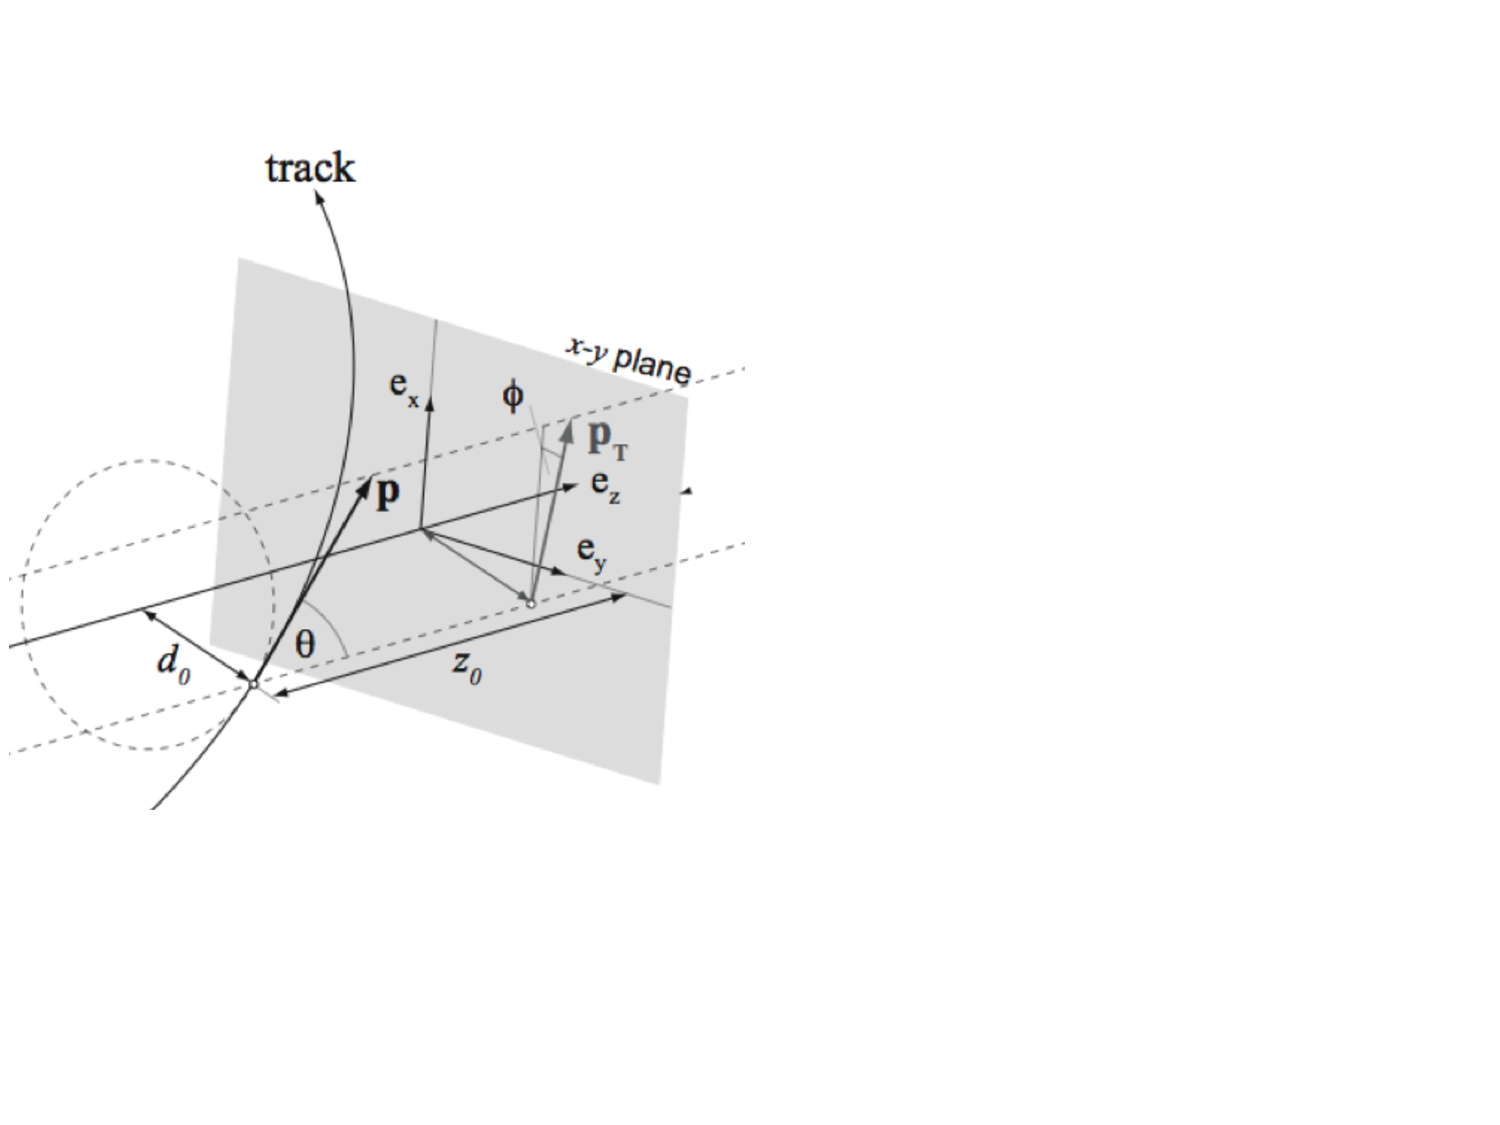
\includegraphics[width=0.8\textwidth]{figures/trkImp.pdf}
	\caption{Illustration of perigee parameters. The most common of these are $d_0$ and $z_0$. The perigee 
may be defined relative to either the beam-line or the interaction point. The analysis in Chapter~\ref{exclH} 
utilizes this choice. Illustration taken from Ref~\cite{ATLAS:trkImp}}
	\label{fig:impctPV}
\end{figure}

\par If a group of tracks reconstructed in the ID are extrapolated to a single spatial 
point in the ID, that point is reconstructed as a vertex. A vertex essentially represents 
a point where a particle, or particles, decay or split into secondary particles that leave 
tracks in the ID. The vertex with the highest sum of track transverse momentum, \pt, is labeled the 
primary vertex (PV). This is the vertex at which the hard scatter occurs. Since the PV does not 
always coincide with the IP, track perigees are usually measured relative to the PV.  

\subsection{Muon Spectrometer Tracks}
\par Seeds for MS track reconstruction are extracted from the precision 
sub-detectors: Cathode Strip Chambers (CSCs) and Monitored Drift Tubes (MTDs).
From MDTs drift circles are processed, and from CSCs {\it clusters} are built.
Signals from drift circles and clusters are used as inputs to pattern recognition algorithms 
to form {\it segments}, which are combined and fitted to form the reconstructed track. 

\par Clusters in the CSCs are muon hits in each chamber that give a 1-dimensional measurement of 
position. Since CSCs are mounted on wheels in the end-caps and are segmented in $\phi$, separate 
$\phi$ and $\eta$ clusters are obtained. A set of clusters is fitted using the Hough transform 
method~\cite{Kiryati:1991:PHT:104022.104026}, which is more suited to fitting non-linear tracks than the Kalman Fitter, to form 
separate $\eta$ and $\phi$ segments. Combining the two gives a 2-dimensional position and a 
direction to each cluster.  

\par Segments in the MDTs are reconstructed from fitting drift circles measured from 
drift tubes in two neighboring stations. Two outer MDT hits are picked as seeds and straight 
lines are fitted between them, accounting for hits in the middle layer. With a minimum of 3 hits 
required to form a segment, the fit with the 
highest number of hits is picked. The quality of an individual hit in an MDT is best described by Figure~\ref{fig:mstrackQ}. 
When the track path perfectly matches the drift radius the MDT is considered to be {\it on track}.
When the drift radius is too small compared to the track path the MDT is referred to as having a {\it $\delta$-electron}.
When the drift radius is too large to match the track, the MDT is considered {\it out of time}, 
and when there is no drift circle the MDT is known as a {\it hole}. A segment is scored by 
$N_{\delta}+N_{out}+N_{hole}$, where the smaller the sum the higher the quality. Ambiguous 
segments are recursively resolved with the score, the $\chi^2$ and the overall 
number of hits. Just like TRT hits, hits from the RPCs and TGCs are fitted to existing segments if they improve 
the segment score. 

\begin{figure}
	\centering
   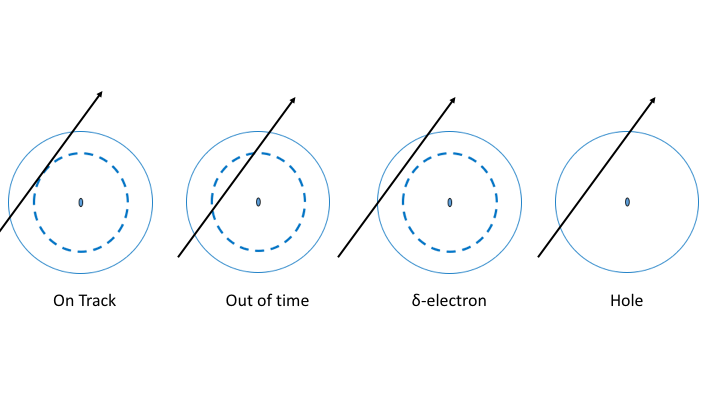
\includegraphics[width=\textwidth]{figures/mstrackMDT.png}
	\caption{Illustration of track fitting in the MS. A track fit to an MDT can be any of 4 cases: track path coincides with drift circle (on track), 
is smaller than drift circle (out of time), is larger than drift circle ($\delta-$electron), and no drift 
circle (hole). Track quality is evaluated by the multiplicity of these cases.}
	\label{fig:mstrackQ}
\end{figure}

\par Full track reconstruction is done by fitting segments, starting from segments farthest 
from the IP and taking into account the bending caused by the 
magnetic field. Each track's $\chi^2$ and number of hits are evaluated and used to 
recursively resolve ambiguities. Finally, the reconstructed tracks are extrapolated to the 
beam-line and their $d_0$ and $z_0$ are extracted. 
    

	
	\section{Electrons}
	\label{sec:ele}
\subsection{Reconstruction and Identification}
\label{sec:eleReco}
\par Electrons reconstructed in the ATLAS detecter are classified into {\it central} 
and {\it forward}, where central electrons are those within $|\eta|<2.5$ and 
forward electrons are those within $2.5<|\eta|<4.9$.
Since central electrons fall within the Inner Detector (ID) coverage, they make use 
of both the EM Calorimeter and the ID measurements while 
forward electrons rely just on the calorimeter information. As a result, calorimeter 
requirements on forward electrons are much more stringent than on central 
electrons.

\par Central electrons are reconstructed by matching energy clusters in the EM Cal 
to tracks in the ID, where a cluster is a group of calorimeter cells.
The slinding window algorithm (introduced in Section~\ref{sec:trigger}) is used 
to find these clusters by searching for calorimeter cells with energy deposits greater 
than 3~\GeV\ in windows of size $3\times 5$ calorimeter cells in $\eta\times\phi$\footnote{
The magnetic field bending plane in the ID is the $r\phi$ plane. The calorimeters may be subject 
to this field as well, albeit significantly weaker than in the ID}. The window 
is made larger in the $\phi$ direction to account for any magnetic field effects. This cluster 
search begins in Layer 2 of the EM Cal. Upon locating the cluster center in Layer 2 energy deposits 
in the corresponding pre-sampler, Layer 1 and Layer 3 are collected and summed. During Run I, using 
the sliding window algorithm, the efficiency for finding electrons with $\eT=7~\GeV$ was 95\% 
, 99\% for those with $\eT=15~\GeV$ and 99.9\% for those with $\eT=45~\GeV$~\cite{Aad:2014fxa}. 

\par Forward electrons are reconstructed using {\it topological clusters}~\cite{Lampl:2008zz}, whose clustering algorithm 
differs from the slinding window algorithm. Cells with large signal to noise ratio are used as seed and 
added to the cluster. The cluster grows by iteratively adding neighboring cells with a signal to noise ratio above a 
threshold slightly less than the seed threshold. Perimiter cells are added on the cluster by 
imposing an even lower energy threshold. This creates 3-dimensional clusters of varying energies. 
During Run I and Run II the seed threshold was 6~\GeV\ and both the neighbor and perimeter 
thresholds were 3~\GeV. This topological clustering scheme is known as EM 633, named after 
energy thresholds from seeds, neighbors and perimeters. 

\par Only tracks with $\pT>0.5~\GeV$, at least 
two hits in the Pixel Detector, at least seven total hits from the Pixel Detector and the SCT are 
considered for matching clusters in the EM Cal. These tracks are extrapolated from 
their last hit in either the Silicon Detectors or the TRT to Layer 2 of the EM Calorimeter.
A track and a cluster are considered a match if the cluster center and the track are within 
$|\Delta\eta|<0.05$ and $|\Delta\phi|<0.1$. The matching window in the $\phi$ coordinate 
is larger to allow for brehmsstrahlung losses due to the magnetic field. In the case of multiple tracks being matched 
to one cluster, preference is given to the tracks with most hits in the Silicon Detectors, based 
on the scoring method discussed in Section~\ref{sec:idtracks}, and the smallest  
$\Delta R$ between the track and the EM Calorimeter cluster. A central electron 
is considered reconstructed if a cluster is matched to a track, otherwise it is reconstructed as 
a photon. To minimize background, only electrons with at least 5~\GeV\ energy are reconstructed. 

\par Effectively, a reconstructed electron is characterized by the following : the cluster energy, the estimate 
of the energy deposited in the ID, EM Calorimeter pre-sampler energy, lateral cluster energy leakage and leakage 
of energy into the hadronic calorimeter. These five components are combined to estimate the total 
electron energy. At $0.5~\MeV$, the electron mass is taken as zero in the ATLAS detector. This approximation 
makes the total electron transverse energy equal to its \pT. 
For central electrons the ($\eta,\phi$) position is extracted from the tracks and  
for forward electrons it is extracted from the topological clusters.   

%\subsection{Identification} 
\par Reconstructed electrons are grouped into categories of several identification 
requirements. The variables that define these categories describe cluster (which in turn describes an electron shower) and 
track properties, as well as criteria used for track-cluster matching. 

\par Of prime importance in describing a shower is the extent of hadronic leakage and the lateral 
shower shape. Given that $\eThadone$ is the transverse energy in Layer 1 of the hadronic 
calorimeter behind the electron cluster, $\eThad$ is the transverse energy 
in the whole hadronic calorimeter section behind the electron cluster, $\eta_2$ is the 
$\eta$ position of the cluster in the EM calorimeter, and $\eT$ is the ratio of the 
cluster energy to $\cosh\eta_2$, the hadronic leakage is defined as 



\begin{equation}
\text{Hadronic Leakage} = \begin{cases} 
														\eThadone/\eT,& \mbox{if } |\eta_2|<0.8 \mbox{ and } |\eta_2|>1.37 \\ 
														\eThad/\eT, & \mbox{if } 0.8<|\eta_2|<1.37  
													\end{cases}
\end{equation}

The lateral shower shape is describe by, among many other variables, $R_\eta(37)$ 
defined as 

\begin{equation}
R_\eta(37) = E(237)/E(277)
\end{equation}
 
where $E(237)$ is the energy deposited in Layer 2 of the EM Calorimeter in a 
rectangle of size $3\times 7$ cell units in $\eta\times\phi$,
centered around the  cluster center. $E(277)$ is similarly the energy deposited 
in a rectangle of size $7\times7$ cell units. Hadronic leakage and lateral 
shower shapes are very efficient in rejecting $\pi^{\pm}$ decays and 
wide showers. To reject electrons from \pizero\ decays Layer 1 of the EM Calorimeter 
is used because of its finer granularity in $\eta$. As already discussed in Section~\ref{sec:trigger} 
\pizero\ decays result in two energy maxima. To search for these two energy maxima several 
variables are defined in a $0.125\times0.2$ $\Delta\eta\times\Delta\phi$ window around the cell 
with the highest energy deposit (the so-called hottest cell). Given that $E_{2nd}$ is 
the energy deposited in the second hottest cell, that $E_{min1}$ is the energy deposited 
in the cell with the least energy between the hottest and second hottest cell, 
$\Delta E = E_{2nd}-E_{min1}$ is an excellent variable for picking up the two 
energy maxima due to \pizero s.  

\par While calorimeter shower analysis significantly reduces backgrounds due to
charged hadron decays, background due to photon conversions are better reduced by 
track analysis. First, track quality requirements are demanded on candidate electron 
tracks: at least nine Pixel Detector hits where one of the hits must be in the B-layer, 
and the transverse impact parameter either with respect to the beamline or to the primary vertex 
is demanded to be less than a threshold value.  
To ensure track-cluster matching, in addition to the $\Delta\phi, \Delta\eta$ requirements 
discussed in the preceding section, the energy measurement from the calorimeter is 
compared to the \pT\ from the track bending. 

\par Categorization of electron identification is successive and inclusive. This means that first 
a category with minimal requirements is defined; latter categories are just sub-sets of the first 
category, with more stringent requirements. The categories are a trade-off between the signal 
efficiency (ratio of identified electrons to reconstructed electrons) and background 
rejection. Reconstructed electrons that pass the first category requirements are referred to 
as {\it loose}. Subsequent categories are referred to as {\it medium} and {\it tight}. 
In general loose electrons pass hadronic leakage and lateral shower shape requirements.   
Medium electrons are additionally pass shower shape requirements in Layer 1, reducing 
\pizero\ contamination. Tight electrons additionally use track quality and track matching criteria 
to reduce backgrounds due to photon conversions. 

\par Rather than directly imposing requirements 
on variables to distinguish between signal electrons and 
background objects, a multivariate technique is used for electron identification for analyses described in 
this text. The discriminant used is the log-likelihood function $\log{d_{\mathcal{L}}}$~\cite{ATLAS-CONF-2014-032}, 
where 

\begin{equation}
d_{\mathcal{L}} = \frac{\mathcal{L}_S}{\mathcal{L}_S + \mathcal{L}_B}, 
\label{eq:lglh}
\end{equation}

where $\mathcal{L}_{S,B}$ are likelihood functions on signal electrons and background objects 
respectively. The $\mathcal{L}_{S,B}$ are functions of probability density functions (pdf) obtained by training a 
multivariate classifier on signal electrons or background objects from Monte Carlo simulations  
using variables discussed in the preceding paragraphs as inputs. A generalization of 
a likelihood function is 

\begin{equation}
\mathcal{L}(\vec{x}) = \prod_{i=1}^{n} P_i(x_i)
\label{eq:lhf} 
\end{equation}

where $\vec{x}$ is a tuple of input variables and $P_i$ is a pdf for variable $i$. 
Categorization into identification categories is achieved by directly cutting on 
$\log{d_{\mathcal{L}}}$, where $d_{\mathcal{L}}$ is computed using successively 
more variables for loose, medium and tight categories.
 
\subsection{Measurement of efficiencies, corrections and uncertainties}
\label{sec:eleCorr}
\par This section quantifies the performance of the electron reconstruction and identification methods 
discussed so far. 

\subsubsection{Efficiency}
\par Electron identification and reconstruction suffers from inefficiencies due 
to detector limitations. These inefficiencies are measured in data and in Monte Carlo 
simulation and compared, ultimately correcting the Monte Carlo simulation predictions. 

\par The total efficiency of reconstructing and identifying electrons for use in an 
analysis can be factorized into its major components as  

\begin{equation}
\epsilon_{total} = \epsilon_{reco} \times \epsilon_{id} \times \epsilon_{trigger} \times \epsilon_{isolation}
\end{equation}

where $\epsilon_{reco}$ is the efficiency of reconstructing an electron once an 
electromagnetic cluster is found in the EM Calorimeter, and $\epsilon_{id}$ is the 
efficiency of categorizing the reconstructed electron as loose, medium or tight.
$\epsilon_{trigger}$ is the efficiency of an identified electron to pass a particular 
trigger and $\epsilon_{isolation}$ is the efficiency of an electron that has passed the trigger 
to pass an isolation selection criteria. These efficiencies are computed successively. For example, 
an electron that passes the trigger selection must have also passed identification, and 
reconstruction. $\epsilon_{reco}$ is particularly 
important because it quantifies track reconstruction and track-cluster matching. 
Electrons, at a mass of $0.5~\MeV$, suffer more from brehmsstrahlung as they 
traverse material in the ID than heavier particles. This results in unpredictable 
deviations in the electron track path in the ID, leading to relatively 
poor reconstruction. $\epsilon_{id}$ on the other hand quantifies the perfomance 
of the Log Likelihood function described in the previous section. This section 
discusses the method for extracting $\epsilon_{id}$ and $\epsilon_{reco}$. 

\par For studies discussed in this text $\epsilon_{id}$ and $\epsilon_{reco}$ were extracted from \Zee\ and 
and \Jee\ events in data to cover a wide electron $\pT$ range. 
In both these cases, the {\it tag-and-probe} method was utilized~\cite{Aad:2011mk}. Here, one 
electron was fully reconstructed and identified with the highest efficiency 
possible. This is known as the tag electron. The other electron was used to 
probe the selection efficiency in question by requiring it to satisfy conditions 
either before or after the selection was been applied. For \Zee\ events, 
the tag electron was tightly identified, matched to a tight trigger electron, had $\eT>20~\GeV$ and  
lied outside the calorimeter transition region ($1.37<|\eta|<1.52$).
For \Jee\ events the tag electron was tightly identified, matched to a tight 
trigger electron object and have $\eT>5~\GeV$. In both cases, a tag object was required 
to be present, with a quality dependent on the type of efficiency being measured. 
For \Zee\ events, \mT\ of the probe object and the tag electron was required to lie between 80 and 100~\GeV.

\par To evaluate systematic uncertainties in the efficiencies being measured, several 
efficiency measurements with variations on the event selection criteria were 
performed. For example, the tag electron was modified or the background estimation 
was varied.  

\par For $\epsilon_{id}$ a reconstructed electron was used as a probe.
In \Zee\ events this probe electron had to have $\eT>10~\GeV$. 
Measurements were extracted from two dimensions: electron \eT\ and  
$\eta$. The decision to bin measurements in $\eta$ was motivated by the fact that brehmsstrahlung 
losses depend on the amount of material that the electron traverses in the ID, which is in turn 
dependent on $\eta$. Results from \Zee\ and \Jee\ events were combined, including systematic 
uncertainties. Figure~\ref{fig:idEff} shows these efficiencies binned 
in \eT\ and $\eta$, in both Monte Carlo simulation and data.  
In general, Monte Carlo simulation modelling agrees reasonably with data. 
The background rejection was also observed to be as large as 400. 

\begin{figure}[h]
\begin{subfigure}{0.5\textwidth}
   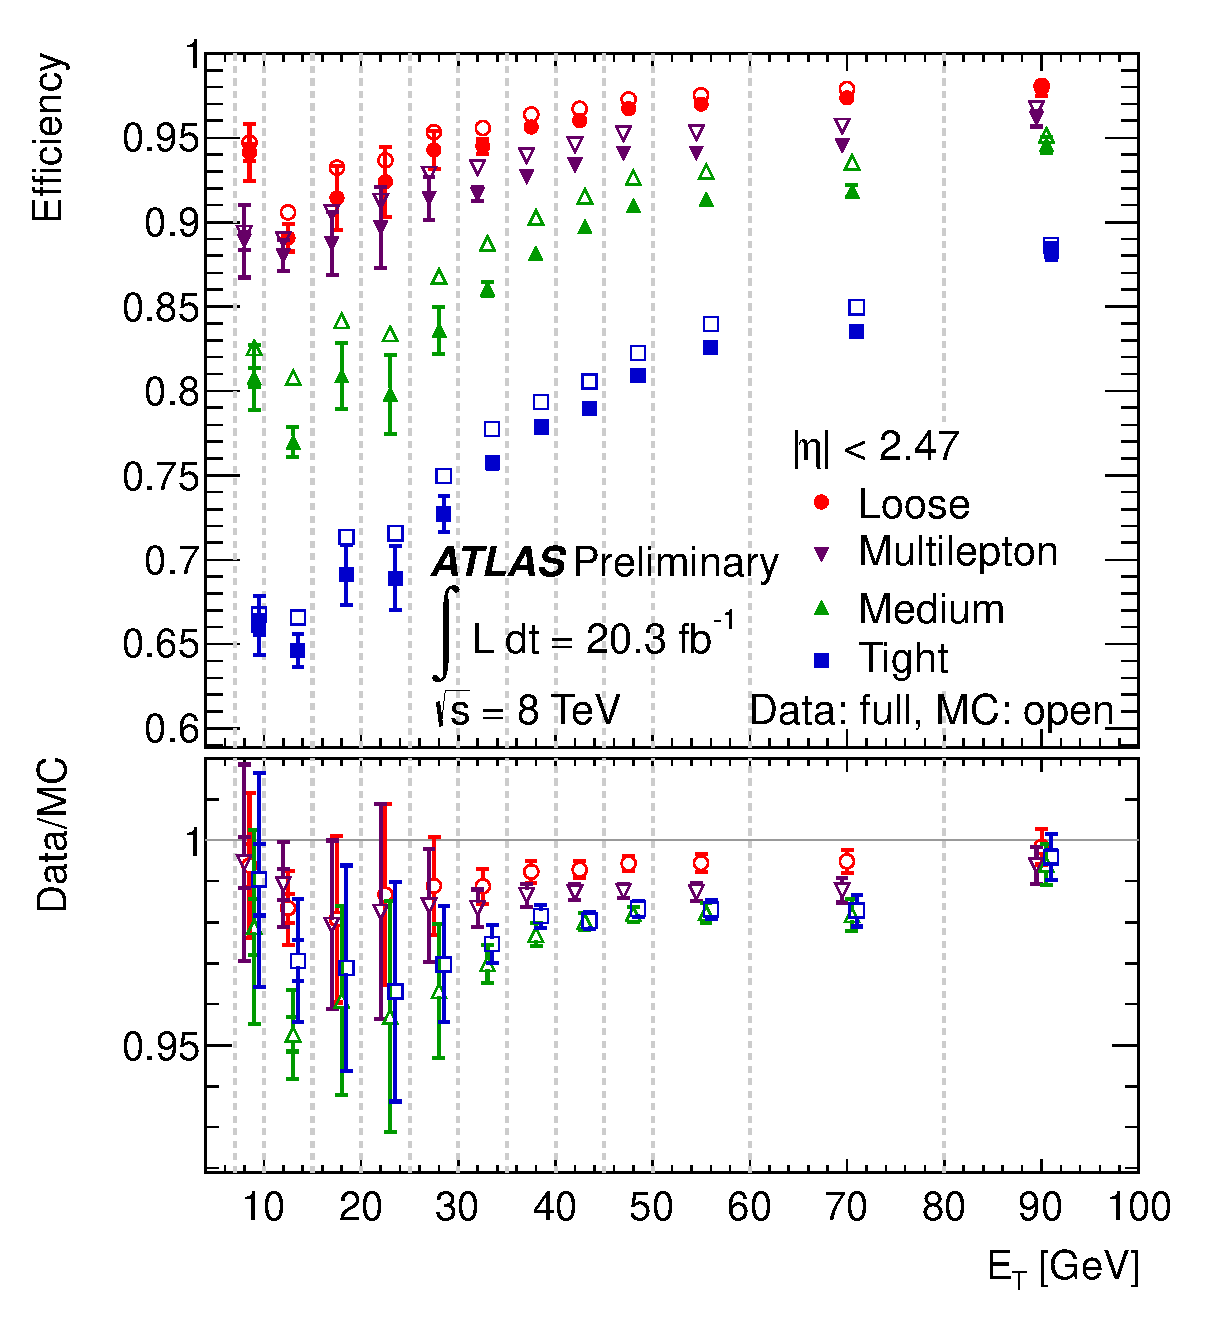
\includegraphics[width=\textwidth]{figures/can_CompEffDataMCLooseMultileptonMediumTightall_0.eps}
	\caption{\eT}
\end{subfigure} % 
\begin{subfigure}{0.5\textwidth}
   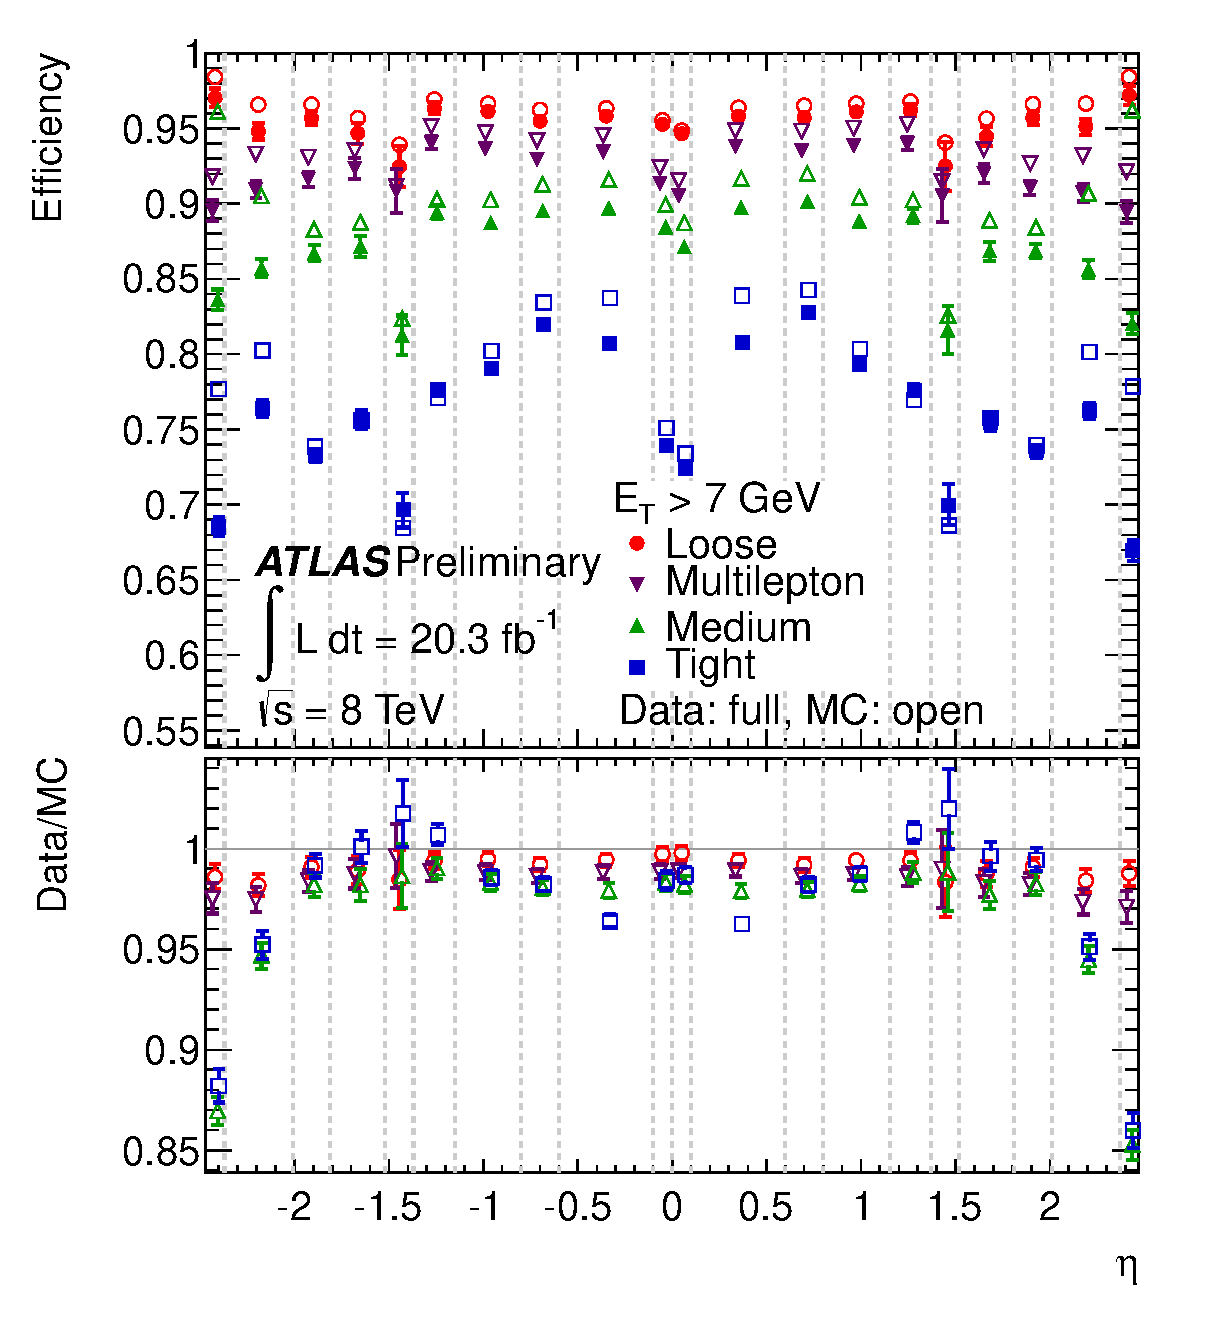
\includegraphics[width=\textwidth]{figures/can_CompEffEtaDataMCLooseMultileptonMediumTightone_0.eps}
	\caption{$\eta$}
\end{subfigure}
\caption{Plots of electron identification efficiencies during Run 1, binned in \eT, and $\eta$. 
Taken from Ref~\cite{Aad:2011mk}}
\label{fig:idEff}
\end{figure}

\par To measure $\epsilon_{reco}$ with \Zee\ events an EM cluster was taken as the probe 
object. This cluster was required to be isolated from electrons, to reduce backgrounds from 
photons. Measurements were binned in \eT\ and $\eta$. Figure~\ref{fig:recoEff} shows the 
measurements obtained data and Monte Carlo simulations. Overall there is reasonable 
agreement between data and Monte Carlo predictions. For the data set used for the analysis in this 
text (2012), the reconstruction efficiencies are at least 90\%.   

\begin{figure}[h]
\begin{subfigure}{0.5\textwidth}
   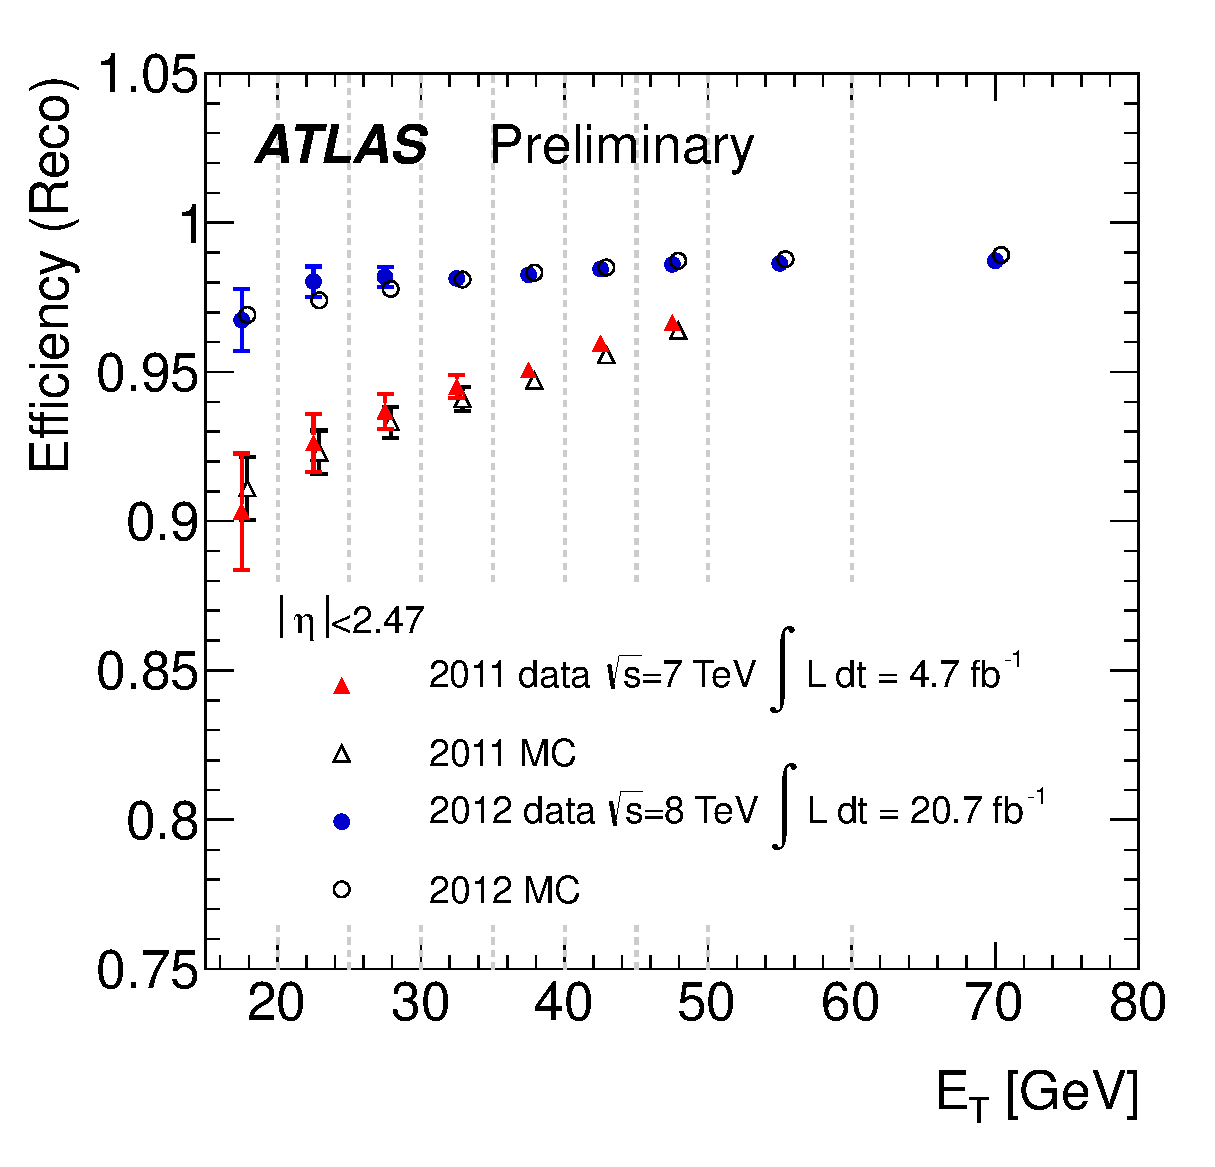
\includegraphics[width=\textwidth]{figures/Reco_et.eps}
	\caption{\eT}
\end{subfigure} % 
\begin{subfigure}{0.5\textwidth}
   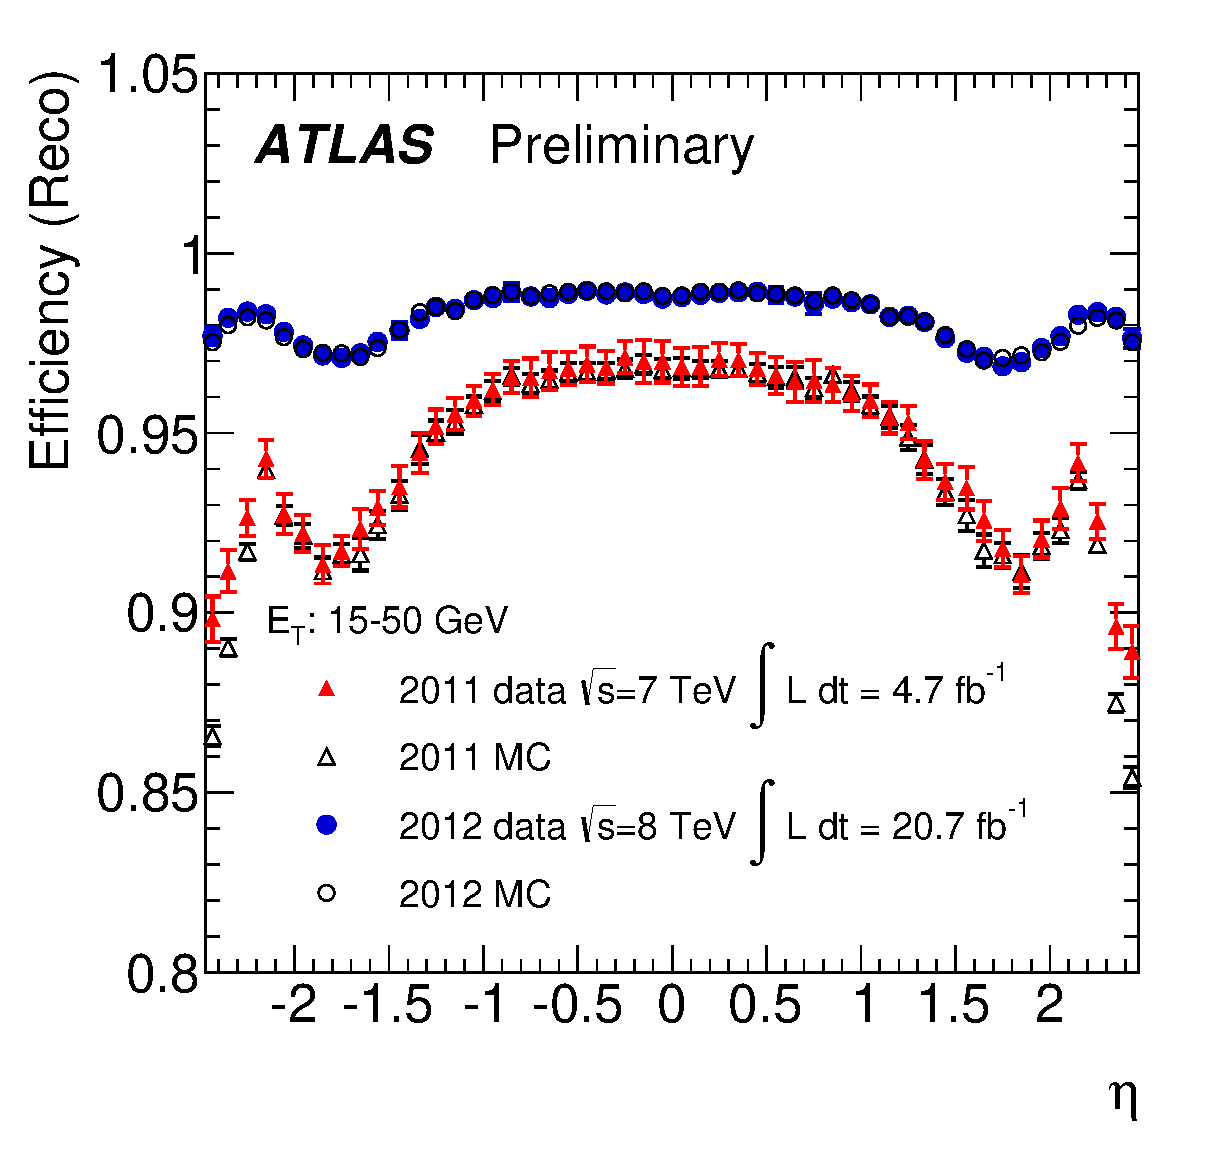
\includegraphics[width=\textwidth]{figures/Reco_eta.eps}
	\caption{$\eta$}
\end{subfigure}
\caption{Plots of electron reconstruction efficiencies during Run 1, binned in \eT, and $\eta$. 
 Taken from Ref~\cite{Aad:2011mk}}
\label{fig:recoEff}
\end{figure}


\subsubsection{Calibration}
\par Electron energy loss in the material upstream or beyond the Lar calorimeters, or outside 
the EM cluster in $\eta$ and $\phi$, was corrected for using dedicated calibration schemes. 

\par To determine these calibration parameters, a Boosted Decision Tree (BDT) was trained on Monte Carlo 
simulation to predict the true electron energy $E_{\text{true}}$ from variables such as the EM cluster 
energy, position, leakages, and ratios of cluster energies in different layers of the Lar calorimeters. 
The training was categorized by $\eT$ and $\eta$, whose binning were chosen to optimize energy responses 
in different regions of phase space. Calibration using this BDT was shown to improve energy 
resolutions by 10\%~\cite{Aad:2014nim}.  

\par Several other corrections were applied to electron candidates after the BDT calibration. For example, 
the energy scales in the first and second layers of the Lar calorimeters were equalized between data 
and Monte Carlo simulation. After that, the overall electron energy response in data was 
calibrated so that it agreed with the expectation from simulation using $\Zee$ events. These calibrations 
were categorized in $\eta$. The sensitivity of the results was evaluated by varying the event selection 
in data, and the quality of the electrons used. 

\par After all these calibrations were applied the agreement between 
data and Monte Carlo simulation was validated in $\Jee$ events, to test the performance in 
a different $\eT$ regime. Figure~\ref{fig:calibVal} shows the invariant masses of the $ee$ 
system in $\Jee$ and $\Zee$ events, covering different $\eT$ regimes. In the \Zee\ case, distributions from data was 
compared to those from calibrated Monte Carlo simulation and uncalibrated Monte Carlo simulation.  
In the \Jee\ case, some of the background component was data-driven, so the calibrated data was 
compared to the sum of Monte Carlo simulation and the data-driven background. 
In both cases, agreement was within 2\%. 

\begin{figure}[h]
\begin{subfigure}{0.5\textwidth}
   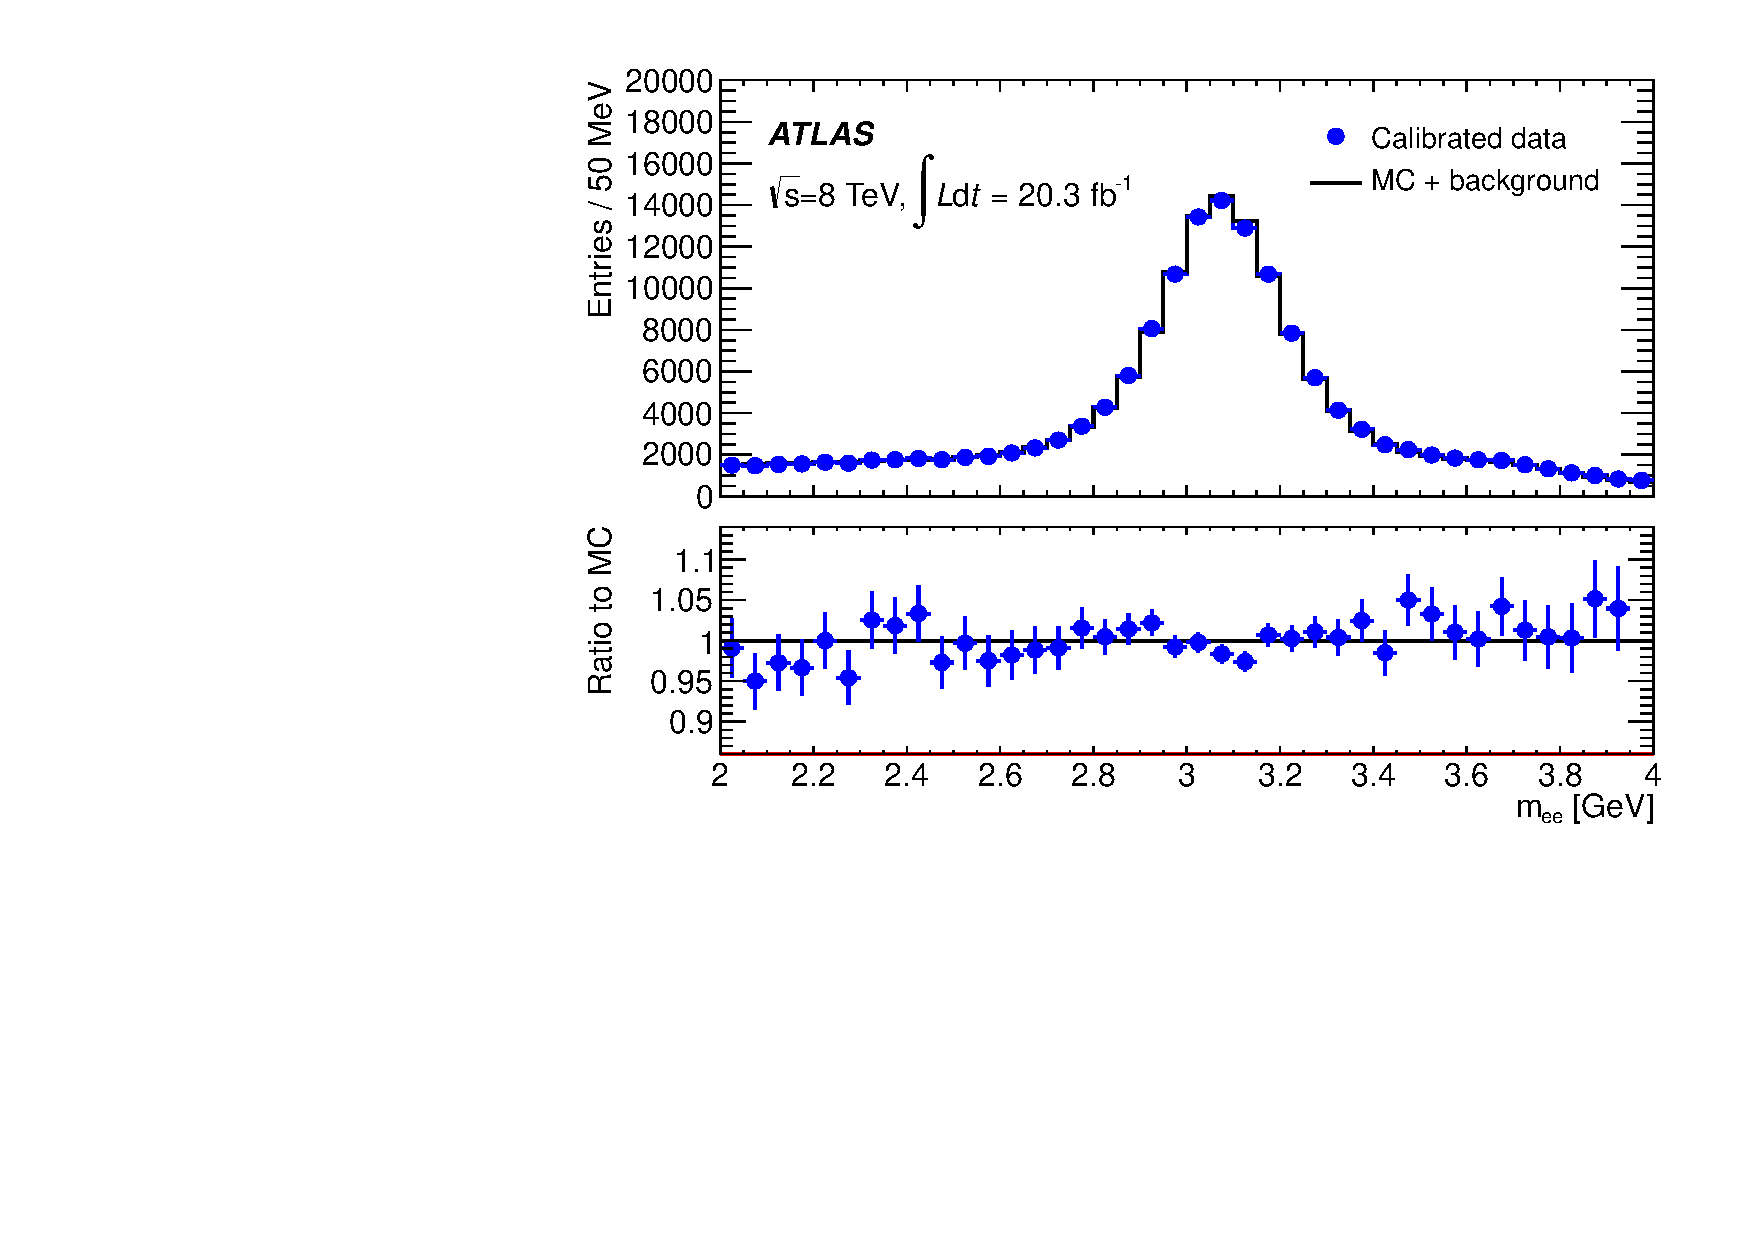
\includegraphics[width=\textwidth]{figures/JPsiPlot.pdf}
	\caption{\Jee}
\end{subfigure} % 
\begin{subfigure}{0.5\textwidth}
   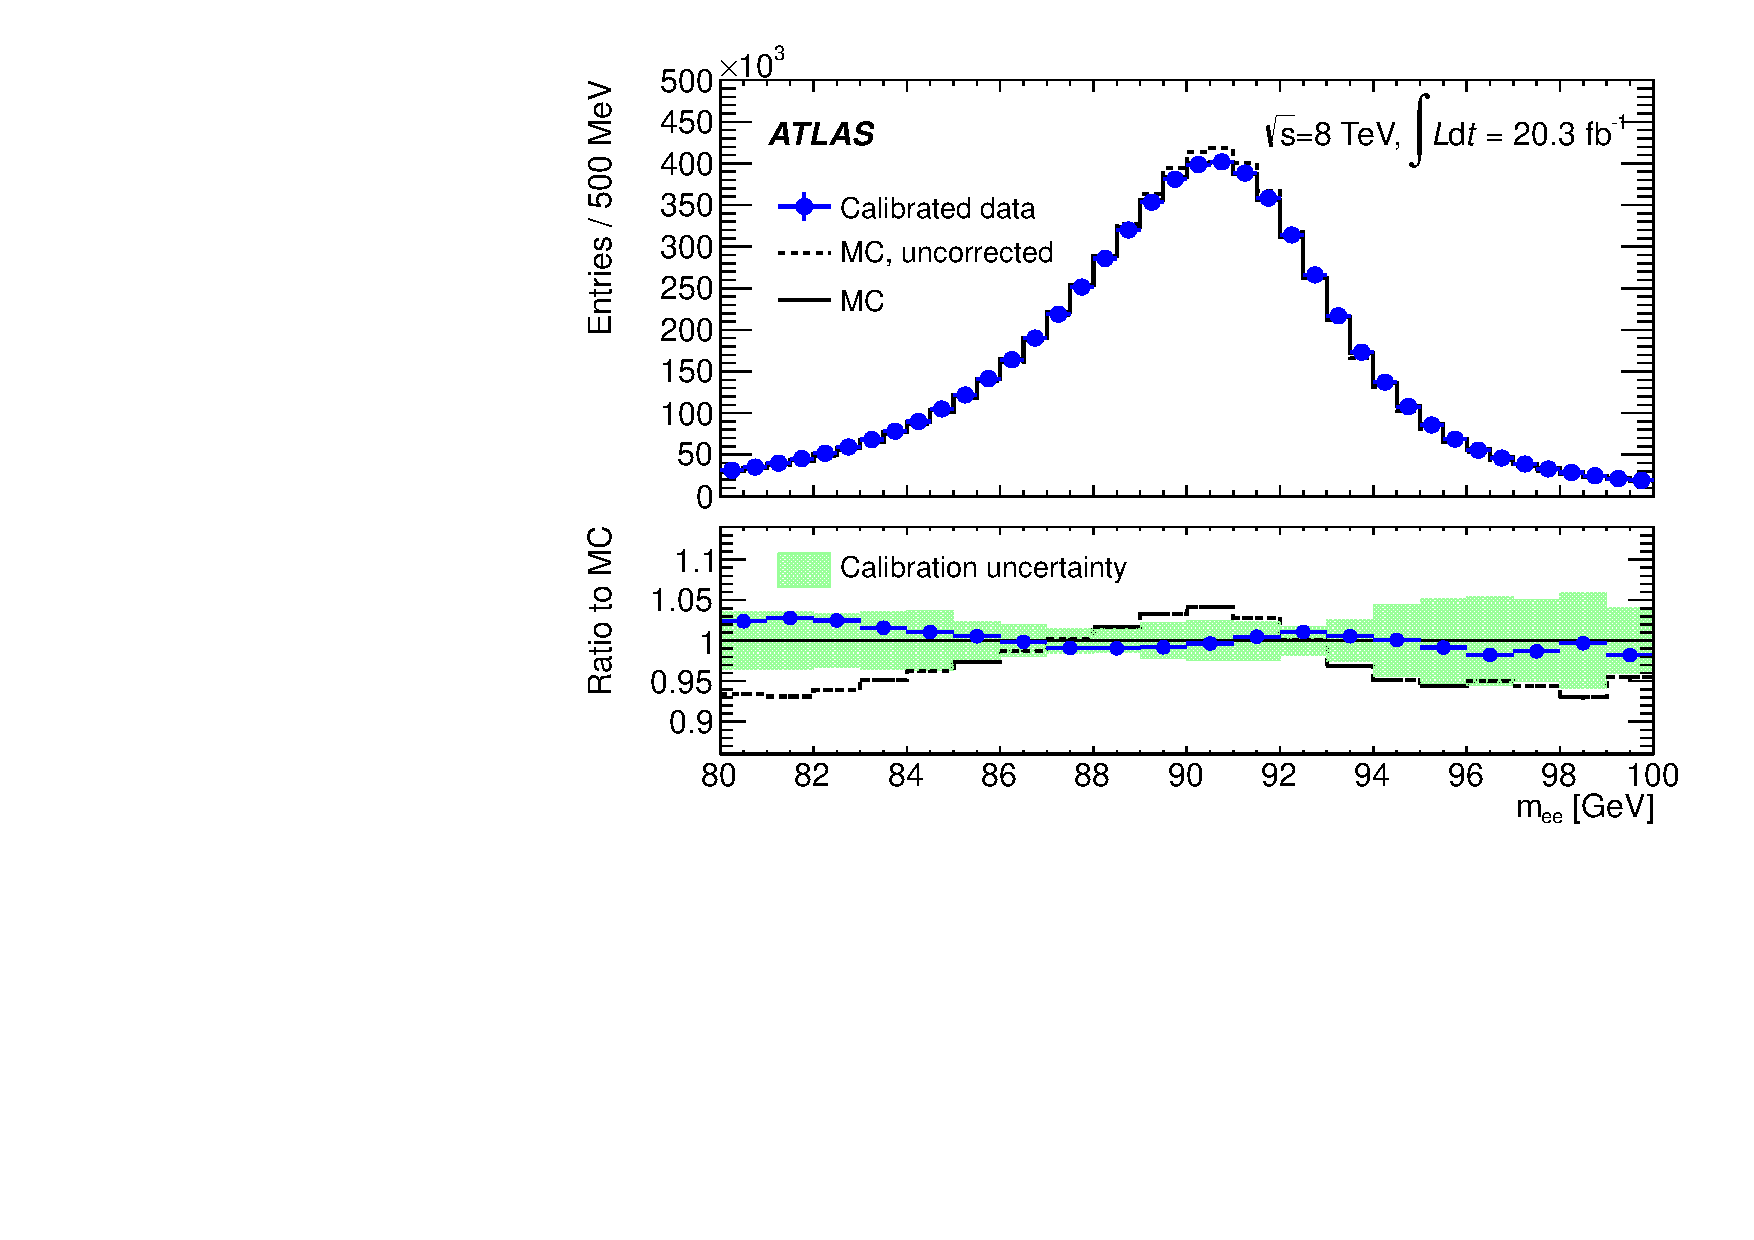
\includegraphics[width=\textwidth]{figures/LineShapePlot_NotZoomed_ForPaper_v3.pdf}
	\caption{\Zee}
\end{subfigure}
\caption{Plots of the invariant mass of the $ee$ system in $\Jee$ and $\Zee$ events in data, calibrated and uncalibrated 
 Monte Carlo simulation. Taken from Ref~\cite{Aad:2014nim}}
\label{fig:calibVal}
\end{figure}

\par Uncertainties in the electron energy scale stemmed from several sources. For example, uncertainties associated 
with calibrating individual Lar layers reached 0.15\%. Those associated with the distribution of material upstream
 the Lar reached 0.3\%. Added in quadrature, overall the uncertainty on energy scale varied from 0.04\% to 0.4\% depending 
on $\eta$. Forward electrons suffered the most. The relative uncertainty on energy resolution was better than 10\% for 
50~\GeV\ electrons, and asymptotically rose to 40\% for higher energies.   
	

	\section{Muons}
	\label{sec:mu}
\subsection{Reconstruction and Identification}
\label{sec:muReco}
\par Every track reconstructed in the Muon Spectrometer is considered a muon track, 
after all ambiguities are resolved. Each of these tracks is further categorized into 
classes upon demanding further identification requirements. Muons identified 
just by tracks from the Muon Spectrometer are classified as {\it Stand-Alone 
Muons (SA)}. As mentioed in Section~\ref{sec:tracking} these tracks are extrapolated to the IP, 
and energy losses from minimal ionizations in the calorimeters are corrected for. 
Muons constructed by combining and matching tracks from the MS and the ID are 
known as {\it Combined (CB)} muons. The overall quality of CB muons is characterized by the significance of 
the ratio of the track charge to its momentum $q/p$, the $\chi^2$ of the combined 
MS-ID fit, and the number of ID track hits. For an ID track to be considered as 
a candidate for matching with an MS track it is required to have at least 1 hit 
in the Pixel Detector, 5 SCT hits, and fewer than 3 Pixel Detector or SCT holes. 
Other types of muons that are rarely used are {\it Segment Tagged (ST)} and 
{\it Calorimeter Tagged (CT)} muons. An ST muon is reconstructed if at least one 
of the MS segments is matched to an ID track, while a CT muon is reconstructed if 
some energy deposits consistent with a muon path in the calorimeters are matched 
to a track in the ID. Purity in these muon classes is ranked as follows: CB, ST, 
SA and CT. Overlaps between classes are resolved in the same order 
of preferrence. CB muons were used in both analyses discussed in this Thesis while 
SA muons are normally used to determine the efficiency of measuring muons with the 
ID. 

\par CB muons used in Run I were required to have at least 3 MDT hits in at least two 
layers. This rule was relaxed to at least 1 MDT layer  and no more than 1 MDT hole in 
the region of $|\eta|<0.1$, which is partially equipped because of service cables.
During Run II muon classes were modified to mimic electron identification classes, 
i.e Loose, Medium and Tight. These classes contain more than one of the CB, ST, SA and 
CT categories. For example, the Medium class is a combination of CB and SA muons. 
For $|\eta|<2.5$ CB muons are used with the same requirements demanded during Run I. For 
$|\eta|>2.5$, which does not have ID tracking, SA muons are used. They are required to have 
hits in at least 3 MDT or CSC layers, and the significance of their $q/p$ is required to be 
less than 7 to reduce contamination from muons from \kaon and  
and \pipm\ decays. Medium muons are used in this Thesis for Run 2 data and CB muons 
are used for Run 1 data.   

\subsection{Measurement of efficiencies, corrections and uncertainties}
\par Just like electron reconstruction, muons reconstruction suffers from inefficiencies 
and energy skews, especially in Monte Carlo simulation. Identification efficiencies in Monte Carlo 
are also not expected to match with those in data.  
Techniques to correct for this are discussed here. 

\subsubsection{Identification Efficiency}
\par Identification and reconstruction 
efficiencies for muons are terms used rather inter-changeably. This 
is because as mentioned before, any track reconstructed in the MS and 
matched to a track in the ID is considered a muon. So, the only efficiency described 
in this text for muons is the identification efficiency, $\epsilon_{id}$. 
Only $\epsilon_{id}$ for muons with $|\eta|<2.5$ is discussed here. Otherwise, the reader 
is encouraged to read Ref~\cite{Aad:2014rra}. For a thorough discussion of muon 
isolation efficiencies the reader is also encouraged to read the same reference.  

\par Since muons with $|\eta|<2.5$ are measured from 
both the ID and MS tracks, the tag-and-probe method is naturally appealing. Given two muons, 
one is used as the tag object and the other as the probe object. The identification efficiency 
can be factorized as  

\begin{equation}
\epsilon_{id} = \epsilon_{id|ID}\times\epsilon_{ID}.
\end{equation}

where $\epsilon_{id|ID}$ is the efficiency of a muon track in the ID to be identified as a muon\footnote{During Run I 
these categories were just CB, ST, CT, etc. During Run II the standard loose, medium, tight working points were 
used.}, and $\epsilon_{ID}$ is the efficiency of a muon track to be reconstructed in the ID. The latter is efficiency 
is difficult to calculate, so it is approximated by $\epsilon_{ID|MS}$, which is the efficiency of 
reconstructing a muon track in the ID given that it has been reconstructed in the MS.  
Ultimately, the efficiencies in data, $\epsilon_{id}^{data}$, and MC, $\epsilon_{id}^{MC}$, are compared 
by taking their ratio as a scale factor. This cancels out any biases stemming from the tag-and-probe 
method.  

\par To cover a wide range of muon $\pt$, efficiency measurements were performed using both 
\Jmm\ and \Zmm\ events from data and MC. 
For \Zmm\ events the tag muon was required to satisfy the following:
\begin{enumerate}
\item medium quality, loose isolation and have $\pT>24~\GeV$; 
\item impact parameter requirements to ensure that it originated from the primary vertex;
\item and be matched to the muon trigger. 
\end{enumerate}
The probe muon was required to have $\pt>10~\GeV$ and be loosely isolated. 
For \Jmm\ the tag muon was required to have $\pT>5~\GeV$, be of medium ID, and be 
matched to the muon trigger. Additionally, for both \Jmm\ and \Zmm the probe muon
was required to have a fully reconstructed muon within $\Delta R< 0.05$ around its location. 

\par Efficiencies were extracted in bins of $\eta,\phi$ and $\pt$, as described in full detail in 
Ref~\cite{Aad:2016jkr}. Figure~\ref{fig:muEff} shows identification efficiencies exctracted from data 
for medium (Run II) and CB (Run I) muons in the region $0.1<|\eta|<2.5$. The high \pt\ region was 
covered by muons from \Zmm\ events while the low \pt\ region was covered by muons 
from \Jmm\ events. Above about 20~\GeV, the efficiency was observed to be independent from 
the muon \pt. Overall, the agreement between data and Monte Carlo simulation was observed 
to be within 1\%.    

\begin{figure}[h]
\begin{subfigure}{0.5\textwidth}
   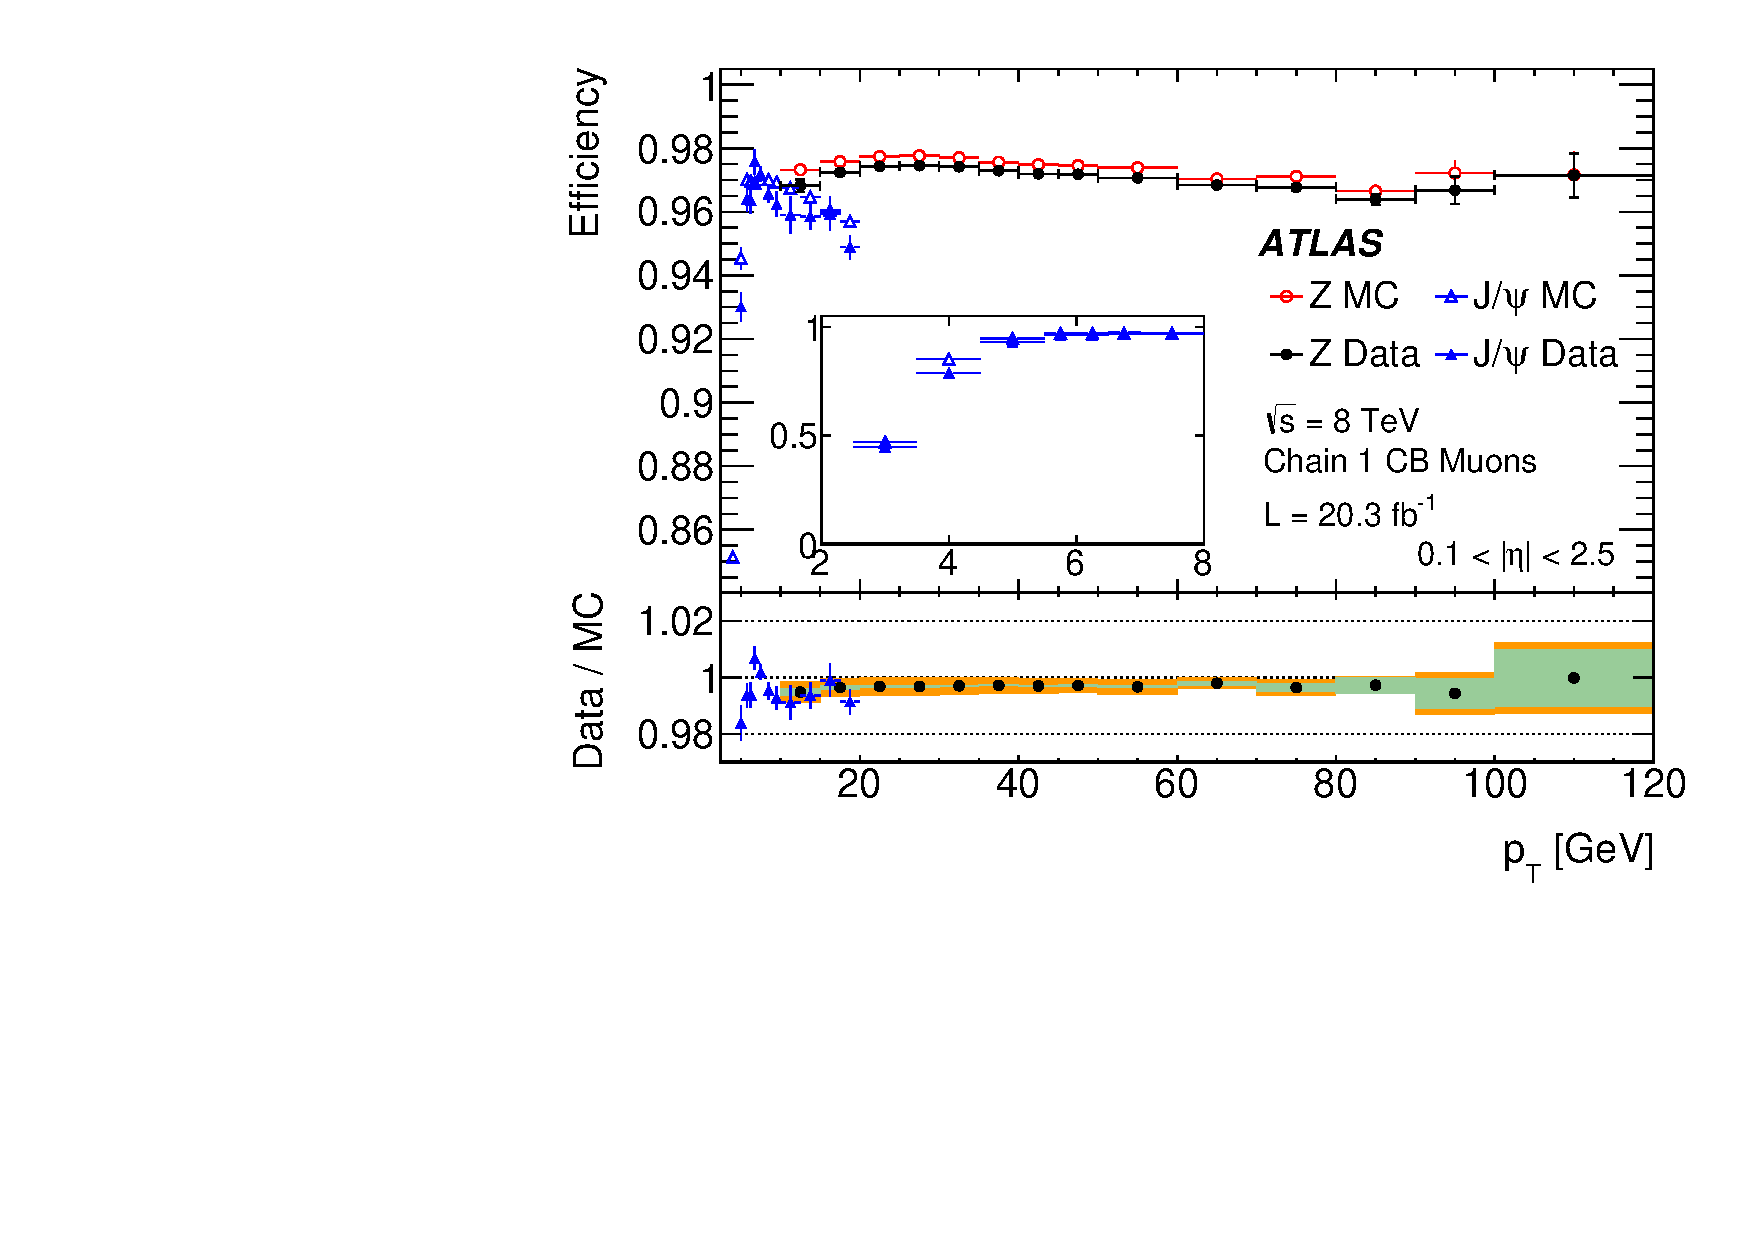
\includegraphics[width=\textwidth]{figures/Full_eff_pt_jpsi_Staco_CB_noCrack.pdf}
	\caption{Run I. Taken from Ref~\cite{Aad:2014rra}}
\end{subfigure} % 
\begin{subfigure}{0.5\textwidth}
   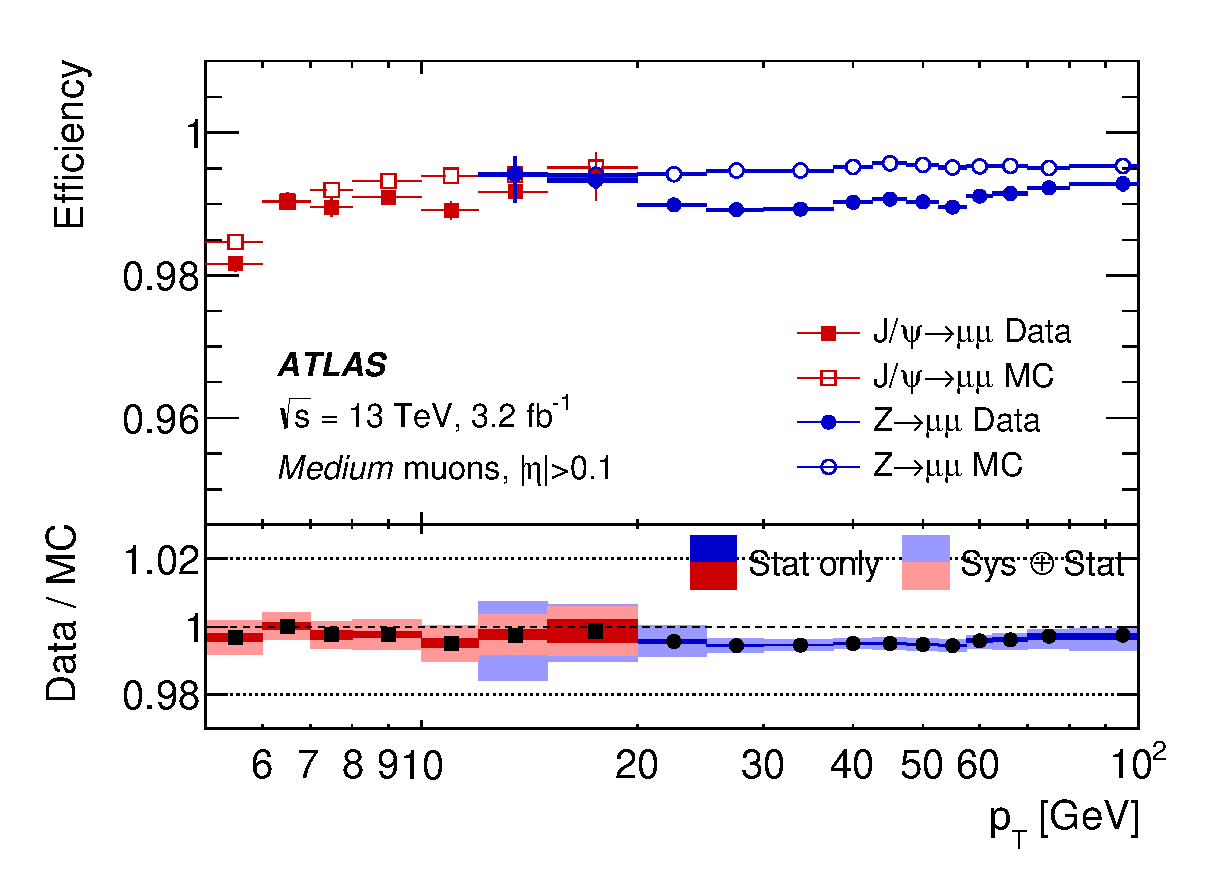
\includegraphics[width=\textwidth]{figures/fig_06.eps}
	\caption{Run II. Taken from Ref~\cite{Aad:2016jkr}}
\end{subfigure}
\caption{Plots of the muon identification efficiencies, binned in \pT. \Zmm\ events were used for high \pt\ muons 
while \Jmm\ events were used for low \pt muons  
}
\label{fig:muEff}
\end{figure}

\par The major systematic uncertainties affecting these results were found to be from the data-driven estimation 
of background processes, choice of cone size used to match probe muons to reconstructed muons, and kinematic 
distribution disagreements between probes in data and Monte Carlo simulation. The uncertainties due to background 
processes was calculated by varying a parameter used in the estimation by $\pm 100\%$. The cone size uncertainties 
were evaluated by varying the cone size by $\pm 50\%$. Distributions of probe kinematics in MC were weighted to 
agree with data. The shift was taken as a systematic uncertainty. After adding these and other~\cite{Aad:2016jkr} 
uncertainties in quadrature, the overall uncertainties on the identification efficiencies were less than 2\%. 
 

\subsubsection{Momentum Scale and Smear} 
\par Just like with electrons, muons may lose energy as they traverse detector material upstream 
of the Muon Spectrometer (MS). This loss may also be mis-modelled in Monte Carlo simulations. 
While losses in the Inner Detector (ID) are very small and taken as negligible, losses the calorimeters 
cannot be neglected. Modelling of the magnetic field integral and detector dimensions in the ID
 and MS in Monte Carlo simulations may also differ from the true physical values. Energy loss and other
forms of mismodelling must therefore be corrected in both data and Monte Carlo simulation. 
Effectively such corrections adjust the muon momentum by scale factors. 

\par Fluctuations in muon energy losses in the calorimeters  
lead to uncertainties in the measured muon momentum. Magnetic field 
inhomogeneities, spatial hits displacements in the ID and MS, and 
misalignment of the MS all lead to larger uncertainties in the measured 
muon \pT\ in both the ID and MS. Accounting for these uncertainties 
broadens (or {\it smears}) the \pT\ resolution in MC to match the data. The corrected muon \pT\ in 
MC can be written as

\begin{equation}
\pT^{corr,MC} = \frac{\pT^{uncorr,MC} + \text{Sum of Scales}}{1 + \text{Sum of Smears}},
\end{equation} 

where the scale and smear corrections are derived from data. 

\par During both Run I and Run II, \Jmm\ and \Zmm\ events from data were used as the source of muons with \pT\ lying in the range 
of 5~\GeV\ to 300~\GeV. Their energy distributions were compared to those predicted by Monte Carlo simulations. 
Muons from \Jmm\ and \Zmm\ were required to be of medium\footnote{In Run I they were required to be CB muons.} 
identification, oppositely charged, within the ID acceptance, and have impact parameters 
that indicate that they originated from the same vertex, which is required to be the primary 
vertex in the event. The invariant mass of the system of two muons,$m_{\mu\mu}$, was required to 
be within 76~\GeV\ and 106~\GeV\ for \Zmm\ and within 2.65~\GeV\ and 3.6~\GeV\ for \Jmm\ events. 
The $m_{\mu\mu}$ distributions were then used to extract correctional scale factors as described in detail in Ref~\cite{Aad:2016jkr}.
Figure~\ref{fig:muScale} shows such distributions for uncorrected MC \pT, 
corrected MC \pT, and data \pT for muons from both \Jmm\ events, using Run I and Run II data-sets. 
These distributions show that a correction for energy losses of about 1\% was necessary. Depending on 
the \pt, resolution smearing corrections below 15\% were applied.     

\begin{figure}[!h]
\begin{subfigure}{0.5\textwidth}
   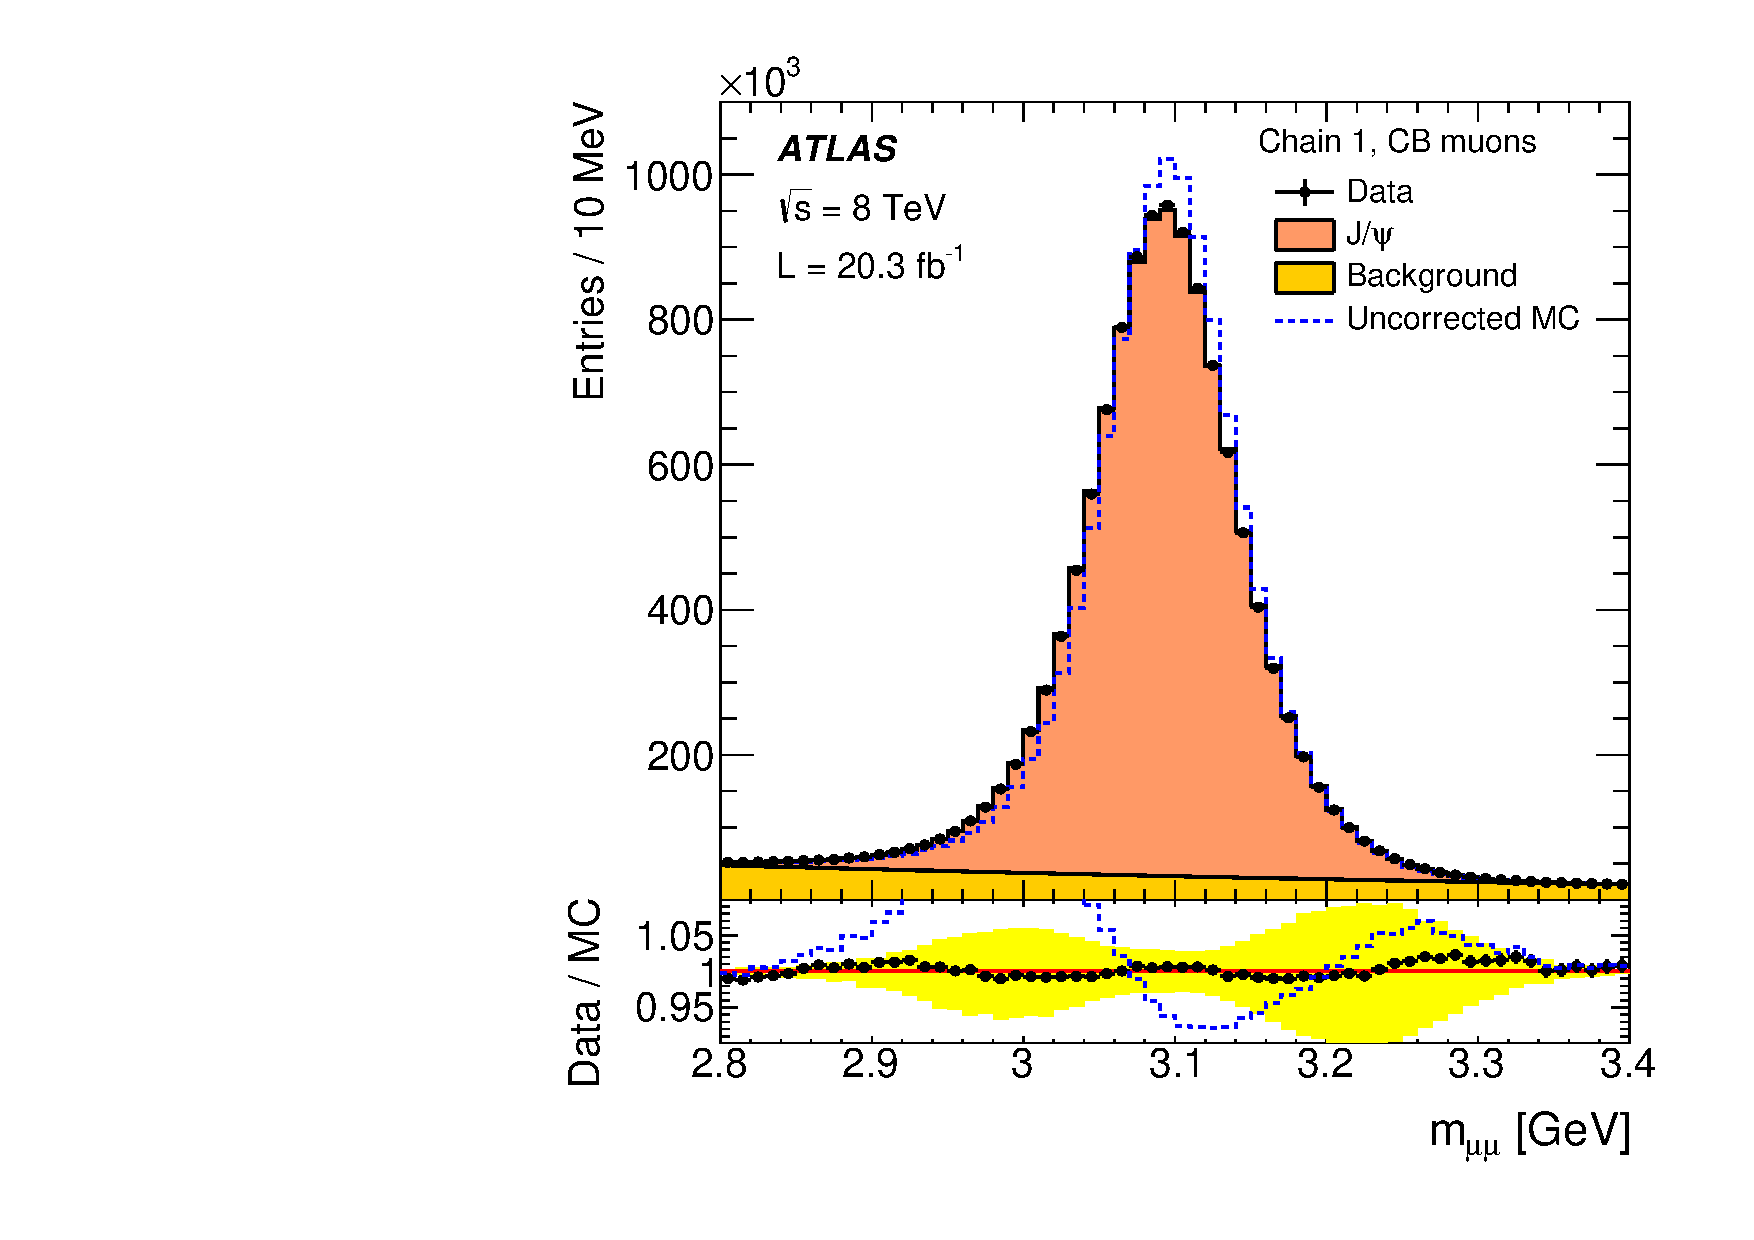
\includegraphics[width=\textwidth]{figures/STACO_jpsi_cb12.pdf}
	\caption{Run I. Taken from Ref~\cite{Aad:2014rra}}
\end{subfigure} % 
\begin{subfigure}{0.5\textwidth}
   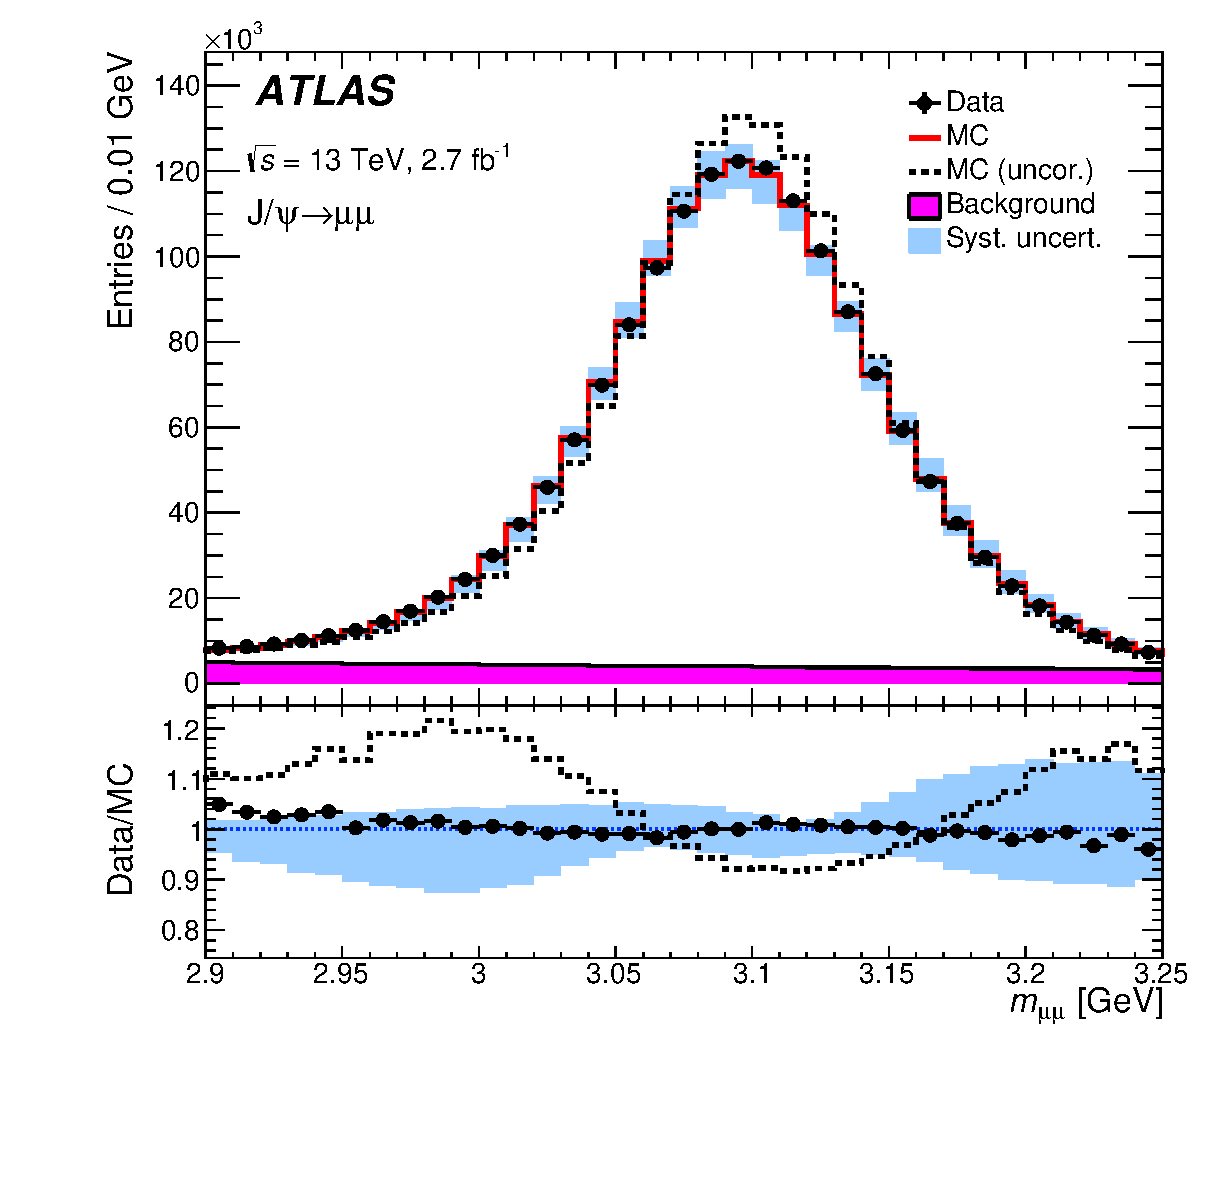
\includegraphics[width=\textwidth]{figures/fig_09_2.eps}
	\caption{Run II. Taken from Ref~\cite{Aad:2016jkr}}
\end{subfigure}
	\caption{Plots showing comparisons of $m_{\mu\mu}$ distributions for muons from \Jmm\ events in data, MC in 
which muon \pT\ is corrected and MC in which \pT is not corrected}
\label{fig:muScale}
\end{figure}

\par Systematic uncertainties in these corrections originate from imperfections in the model 
used for momentum correction, and in the fit used to extract correctional parameters. 
These were evaluated by varying several components when extracting the corrections. For example, the 
$m_{\mu\mu}$ window was varied by $\pm 5~\GeV$ in \Zmm\ event selection. This variation had the most impact 
effect on results.   


	\section{Jets}
	\label{sec:jets}
\par A {\it jet} in the ATLAS detector is a stream of collimated hadrons 
and other particles originating from a localized vertex. Although these jets can be formed from 
hadronic decays of heavy particles such as $W$ or $Z$ bosons, most  
are formed through scattering of gluons and quarks, and radiation of quarks inside the protons during a $pp$ collision.
Jets formed through the latter processes are referred to here as QCD multi-jets. 

\par Due to asymptotic freedom~\cite{Gross:1998jx}, introduced in Section~\ref{sec:qcdTheory}, although 
quarks and gluons cannot move freely at the \GeV\ energy scales, they can move quasi-freely inside the barriers 
of hadrons and baryons. At the LHC hard-scatter energy scales (\TeV) however, quarks and gluons 
may briefly move freely until their energies decrease. During this brief moment, quarks and 
gluons may radiate gluons, and gluons may split into $\qqbar$ pairs, as shown in Figure~\ref{fig:qgVet}.    
This process repeats until a low-enough energy is reached, forming a parton shower. The \qqbar\ pairs 
eventually hadronize to form high energy mesons such as \pipm, neutral and charged \kaon\ that propagate in  
more-or-less the same direction as the direction of the original quark or gluon. 
This collection of hadrons makes up a jet. A formal discussion of parton shower development 
and hadronization is in Sections~\ref{sec:partonShower} and \ref{sec:hadronization}. 

\subsection{The anti-kt clustering scheme}
\par Several schemes have been developed to standardize the mechanism with which  
hadrons are incorporated into a jet~\cite{Glover:1995nx}. The ideal scheme is expected to be insensitive to 
slight modifications to the jets through infrared emmissions or collinear splitting because such modifications 
are stochastic and difficult to predict. Moreover, it is expected to be easy to 
implement in an experimental setting. The jets used in these analyses are defined using the 
{\it anti-kt algorithm}~\cite{Cacciari:2008gp}, which takes topological clusters of calorimeter 
cells as inputs. The energy in the topological clusters corresponds to energy deposited by hadrons 
in the calorimeters.\footnote{
Details on how topological clusters are built from calorimeter cells were 
presented in Section~\ref{sec:ele}.} 

\par The jets are built from two types of topological clusters. For the 
first type, energy deposits in calorimeter cells are calibrated assuming that 
the particle is a neutral pion. This form of calibration is known as the electromagnetic (EM) scale because a neutral pion 
immediately decays to two photons that initiate an EM shower. Although this scale is correct for 
electromagnetic particles, it is not correct for hadrons. The second type of jet corrects for this 
offset in calibration by calibrating hadron energy deposits as if the particle is a charged pion. By first classifying 
each calorimeter cell energy deposit as EM or hadronic, each calorimeter cell is given an independent 
local weight; this process is therefore rightfully called {\it local cell signal weighting} (LCW).
Although LCW is significantly slower than implementing the EM scale, it is a more accurate calibration scale. 

\par Unlike topological clusters for forward electron reconstruction, topological clusters used 
for jet reconstruction use as seed calorimeter clusters with signal to noise ratio of 4.  
Additionally, signal to noise ratio for neighboring cells is required to not be less than 2.
The topological cluster building scheme for jets is therefore 422, while for electrons it is 633.\footnote{
See Section~\ref{sec:eleReco}.}
The definition for noise in calorimeter cells used in both these schemes is the 
sum of electronics noise and energy from pileup $pp$ collisions. 
The pileup component of noise increases with the increase in pileup events. Because of this, 
noise thresholds used during Run 1 jet reconstruction were lower than those during Run 2.
Additionally, during Run 2 topological clusters were not allowed to start building from 
the EM Calorimeter presampler. This significantly reduced the number of jets from pileup 
events.

\par The anti-kt algorithm uses the metric defined in Equation~\ref{eq:antikt} 
to determine cluster association in the position-energy phase space.

\begin{equation}
\begin{aligned}
d_{ij} = \mbox{min}(\pti^{-2},\ptj^{-2})\frac{\Delta R^2_{ij}}{R^2}, &  \mbox{ where } \Delta R^2_{ij}=(\eta_i-\eta_j)^2+(\phi_i-\phi_j)^2 \\
d_{iB} = \pti^{-2} &  
\end{aligned} 
\label{eq:antikt}
\end{equation}  

The second equation in Equation~\ref{eq:antikt} is meant to draw an association between 
a hadron and the incoming or outgoing proton beam, while the first definition assesses the relation 
between two hadrons. The $R$ parameter is a solid angle that limits  
the window of hadron association. During both Run 1 and Run 2, jets were reconstructed with $R=0.4$.
 This metric in Equation~\ref{eq:antikt} is designed to be invariant under boosts in the $z$ 
coordinate because it is made up of $\pT, \eta$ and $\phi$, which are also invariant under similar transformations. 

\par The anti-kt algorithm proceeds as follows, starting with a list of topological clusters :
 The highest \pT\ cluster ({\it the hardest})
is found and indexed with $i$. $d_{iB}$ and $d_{ij}$ are evaluated, where $j$ is the cluster closest 
to $i$, as determined by Equation~\ref{eq:antikt}. If $\min(d_{ij},d_{iB}) = d_{ij}$, $i$ and 
$j$ are combined into a single cluster and the process is repeated, otherwise $i$ is declared 
a final-state jet and removed from the cluster list. This process is repeated until no cluster remains in 
the seed list. The four-momentum of the resultant jet is the sum of the four-momenta from all 
the contributing clusters. 

\par Starting with the hardest cluster, the anti-kt algorithm effectively groups low \pt\ 
clusters around the hardest cluster. This strategy is most convenient at the LHC, where the most important 
jets are usually of high \pt. Additionally, because the metric defined in Equation~\ref{eq:antikt}
includes a combination of an angle and energy it is insensitive to collinear splitting and infrared 
emmissions.  

\subsection{Performance and Calibration}
\label{sec:jetCalib}
\par Jet reconstructed using the anti-kt clustering scheme may have energy offsets due to several 
detector imperfections. These issues are corrected by calibrating several components of the jets. 
The following corrections or calibrations are applied sequentially.

\subsubsection{Origin Correction}
\label{sec:orCorr}
\par Topological clusters positions are computed relative the LHC's interaction point (IP).
Reconstructed jet positions are therefore also computed relative the IP.
Since the primary vertex from which the jet originates may not necessarily 
coincide with the IP, the jet origin has to be adjusted. The scheme proceeds as 
follows: The primary vertex is searched for by selecting the vertex whose 
tracks have the largest sum of \pt. Topological clusters are repositioned to match the 
identified primary vertex. Jet four-momentum is recalculated with the new cluster 
four-momenta. The jet energy response and resolution are not affected by this correction, 
but the jet pseudorapidity resolution is improved. This is expected since the beam spot 
is significantly longer in the $z$ direction (5 cm) than it is in the transverse plane (at most 1 mm). 

\subsubsection{Pileup Subtraction from each jet}
\label{sec:ghosts}
\par The calibration scheme to subtract pileup contamination from each jet is done 
at an event by event, and jet by jet basis. The subtracted quantity in each jet \pt\  
is the product of the jet \pt\ and the event {\it pileup density}, $\rho$, which 
is a measure of how many particles from pileup events were included in the jet. 
The assumption in this scheme is that particles from pileup should be uniformly 
distributed in $\eta\times\phi$. To determine each jet's sensitivity to these particles, 
particles of infinitesimal \pt\ (known as {\it ghost} particles~\cite{Cacciari:2008gn}) are added to 
the event and jet reconstruction is repeated. The number of ghost particles in each jet are used 
to parameterize the area, $A_{j}$, of the jet in $\eta\times\phi$. The median of $\pt/A_{j}$ for all 
the jets in the event is picked as $\rho$ for that event. 

\par Figure~\ref{fig:rho8} shows the $\rho$ 
distributions from simulation events during Run 1, where the number of vertices, $N_{PV}$, 
is varied. The average $\rho$ increases with $N_{PV}$ as expected. The distributions 
shown in Figure~\ref{fig:rho13} are similar to those in Figure~\ref{fig:rho8} but with Run 2 settings.
Any residual dependence of jet \pt\ on $N_{PV}$ and the average number of interactions 
per bunch crossing $\langle\mu\rangle$ is further corrected from bins of $N_{PV}$ and $\langle\mu\rangle$. 

\begin{figure}[h]
\begin{subfigure}{0.52\textwidth}
   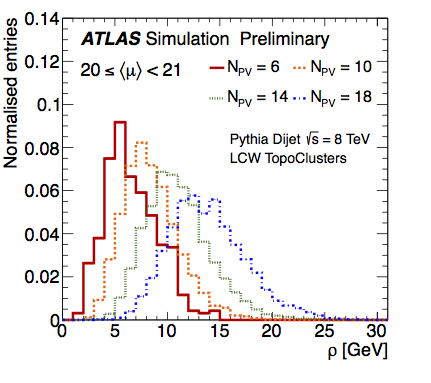
\includegraphics[width=\textwidth]{figures/rho8.png}
	\caption{$\rho$ during Run 1, taken from Ref~~\cite{Malaescu:2048678}}
	\label{fig:rho8}
\end{subfigure} % \hspace{0.2\textwidth}
\begin{subfigure}{0.48\textwidth}
   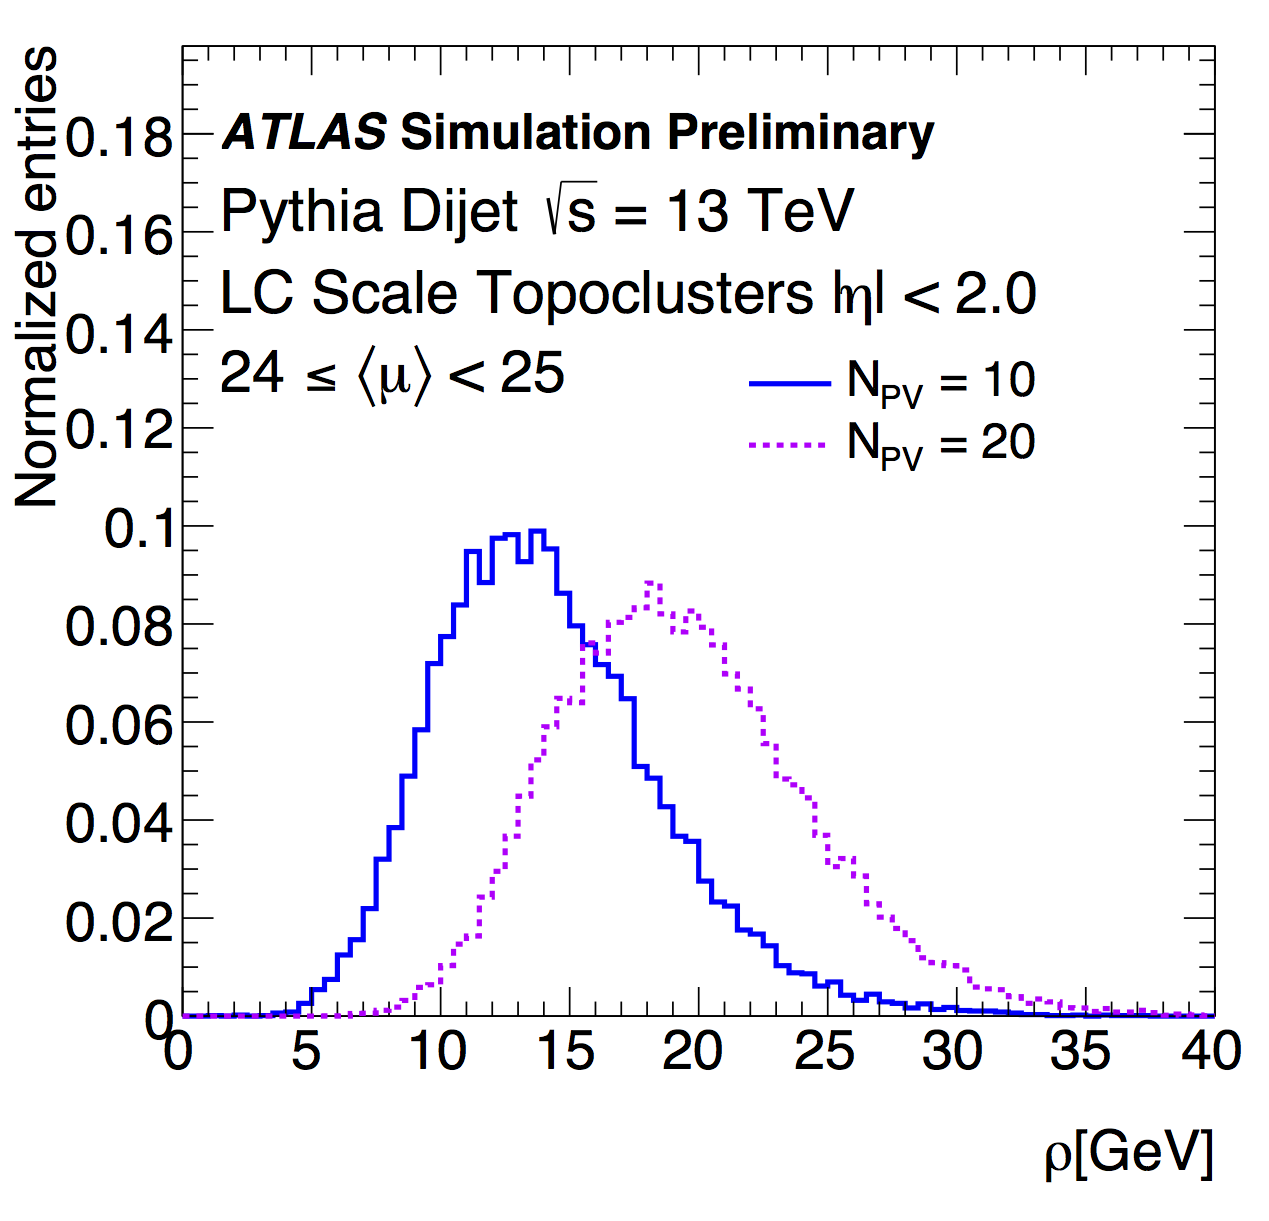
\includegraphics[width=\textwidth]{figures/rho13.png}
	\caption{$\rho$ during Run 2, taken from Ref~\cite{Dandoy:2136864}}
	\label{fig:rho13}
\end{subfigure}
	\caption{Plots showing the pileup density $\rho$, the pileup contribution to jet \pt, 
at several number of vertices $N_{PV}$ for jets reconstructed from LCW topological clusters}
\end{figure}

\subsubsection{Energy Scale and Resolution}
\label{sec:jes}
\par After calibrations schemes described so far have been applied, any remaining jet energy dependence 
on $\eta$ and \pt\ is corrected by comparing the calculated jet energy and the true 
particle jet energy from MC simulation. A jet is matched to a true particle if the true particle 
is within its $\Delta R<0.3$. The jet energy {\it response} (also known as {\it scale}\footnote{These 
terms will be used interchangeably in this text}) $\mathcal{R}$ is defined as the ratio of the 
reconstructed energy $E^{reco}$ to the energy of the true particle jet $E^{true}$. Jet {\it \pt\ 
response} is defined similarly. Jet energy in simulation is finely binned in $E^{true}$ and $\eta_{det}$ bins, 
where $\eta_{det}$ is the pseudo-rapidity in detector coordinates rather than the corrected $\eta$ 
described in Section~\ref{sec:orCorr}. The motivation for $\eta_{det}$ parameterization is that problems may arise from transitioning 
from the barrel to end-cap calorimeters.

\par The jet energy response is measured in bins of $E^{true}$ and $\eta_{det}$. The value in each bin 
is taken as the peak of a gaussian fit for all the values that fall in that bin. 
The energy {\it resolution} is then taken as the standard deviation of the said gaussian 
fit, so it is binned in the same manner as the energy response.  
For each $\eta_{det}$ bin, a calibration function $\mathcal{F}(E^{reco})$ is obtained by a fit of 
$(E^{reco},\mathcal{R})$ values for each $E^{true}$ bin. The corrected jet energy is then 
defined for each $\eta_{det}$ bin as 

\begin{equation}
E^{corr} = E^{reco}/\mathcal{F}(E^{reco})
\end{equation}

where $1/\mathcal{F}(E^{reco})$ is the jet energy scale. A simple approximation, 
$\mathcal{F}(E^{reco}) = \langle E^{reco}/E^{true}\rangle$, was used in both Run I and Run II. 
In this approximation, $\mathcal{F}(E^{reco})$ is the average jet energy response per $\eta_{det}$
bin. Figure~\ref{fig:eResPt} and \ref{fig:eResEta} show the jet energy response for $\pt^{true}$ and $\eta_{det}$ respectively for 
simulated LCW anti-kt jets, with $R=0.4$. The disagreement in the low \pt\ range is caused by non-perfect 
fits which were caused by non-Gaussian effects. 

\begin{figure}[h]
\begin{subfigure}{0.5\textwidth}
   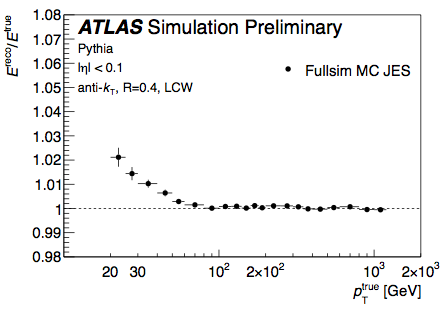
\includegraphics[width=\textwidth]{figures/eResponsePt.png}
	\caption{Jet energy response vs. $\pt^{true}$}
	\label{fig:eResPt}
\end{subfigure} % \hspace{0.1\textwidth}
\begin{subfigure}{0.5\textwidth}
   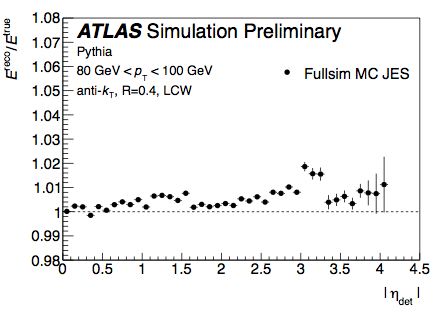
\includegraphics[width=\textwidth]{figures/eResponseEta.png}
	\caption{Jet energy response vs. $\eta_{det}$}
	\label{fig:eResEta}
\end{subfigure}
\caption{Plots showing the jet energy response for simulated LCW jets reconstructed with the 
anti-kt algorithm at R$=0.4$ is plotted against $\pt^{true}$ and $|\eta_{det}|$. 
Taken from Ref~\cite{Malaescu:2048678}}
\end{figure}

\par Studies described in the preceding paragraphs were performed with Monte Carlo simulations 
for several physics processes to evaluate the associated systematic uncertainties. 
These are $Z+$jets, $\gamma+$jets and events with only 2 jets. Jets in the central region were observed 
to have at most 3\% uncertainty in the jet energy scale, and those in the forward regions 
had at most 6\%. The resolution was observed to increase with true \pt\ and with higher pseudorapidity. 
The total uncertainty on the resolution was calculated by varying the Gaussian fits (introduced in this 
section) by $\pm 1\sigma$. This uncertainty was observed to be at most 2\%, varying with the 
true \pt.  

\subsubsection{Jets from pileup}
\par Even after tracks from pileup events that get associated to jets are subtracted with 
the technique described in Section~\ref{sec:ghosts} are subtracted from the jet, jets that originate 
entirely from pileup events are not subtracted from the event. Techniques used to suppress such jets have 
evolved from Run 1 to Run 2. 

\par During Run 1, the Jet Vertex Fraction (JVF)~\cite{TheATLAScollaboration:2013pia} was the main variable used 
to suppress jets from pileup interactions. In an event with multiple reconstructed vertices, 
JVF for a jet was used to determine the likelihood of it originating from each of the 
vertices. Thus, JVF is a function of the jet $\text{jet}_i$ and reconstructed vertex $V_j$ in the 
event. Precisely, it is defined as 

\begin{equation}
\text{JVF}(\text{jet}_i,V_j) = \frac{\sum_m\pt(\text{track}_m^{\text{jet}_i},V_j)}{\sum_n\sum_l\pt(\text{track}_l^{\text{jet}_i},V_n)},
\label{eq:jvf}
\end{equation}  

where $m$ runs over tracks associated with $\text{jet}_i$ and whose origin is $V_j$. $n$ runs over all reconstructed vertices in 
the event and $l$ runs over all tracks whose origin is $V_n$ and associated with
 $\text{jet}_i$. For each of these tracks a $\pt>500~\MeV$ 
requirement is demanded. For jets with no tracks, a value of -1 is assigned to JVF. During Run 1 the vertex of interest was 
the primary vertex, $V_0$. $\text{JVF}(V_0)$ was used as a discriminant for each jet. 
Figure~\ref{fig:jvfPl} shows the $\text{JVF}(V_0)$ distribution for simulation jets from the primary vertex (hard-scatter jets) 
and jets from pileup, for jets with $20<\pt<50~\GeV$ and $|\eta|<2.4$. These jets were reconstructed using the LCW 
scale and the jet energy scale~\ref{sec:jes} (JES) was applied. Pileup jets tend to have low JVF 
because their tracks rarely originate from the primary vertex. Using $\Zmm+$jets events from simulation 
it was observed that pileup jets during Run 1 were suppressed to $2\%$ for jets with $\pt\approx20~\GeV$ 
and even to lower values for jets with higher \pt. 

\begin{figure}[!h]
\centering
   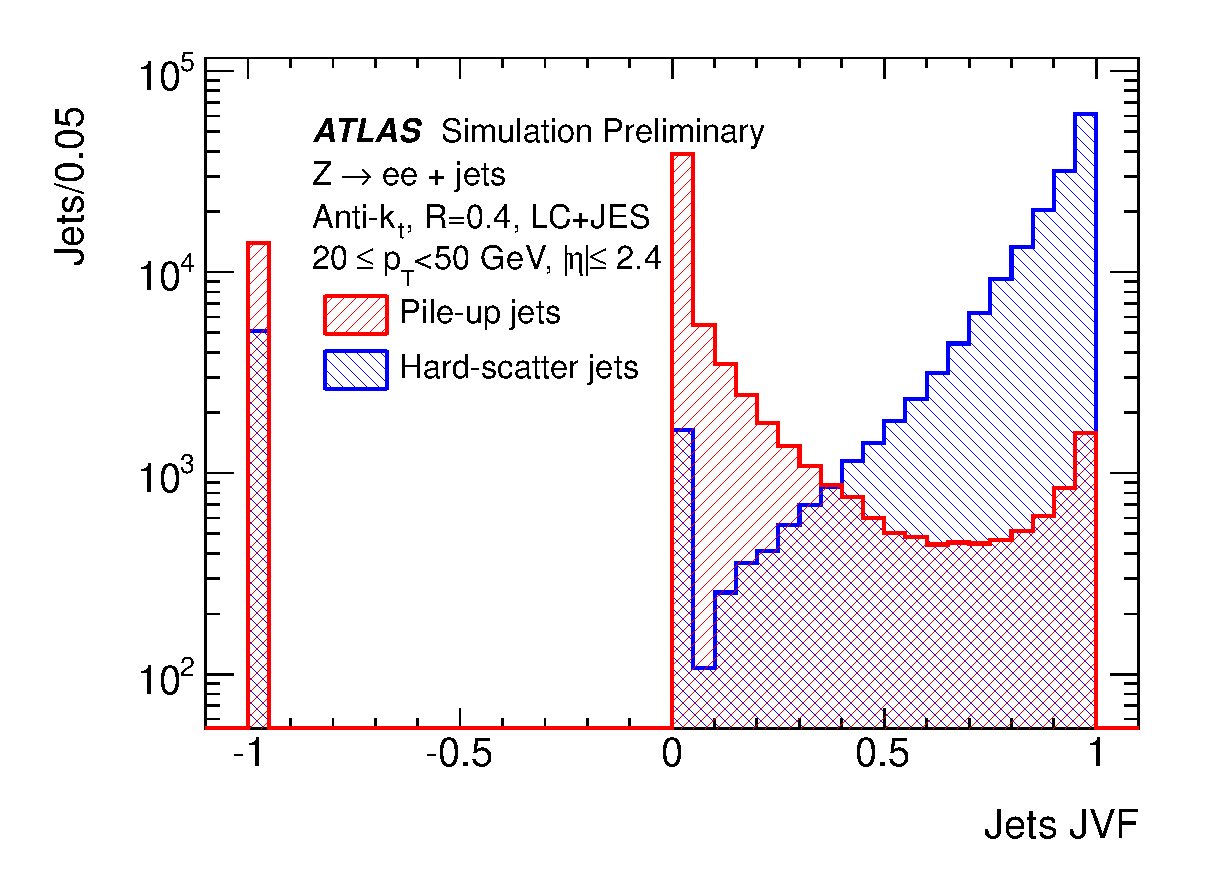
\includegraphics[width=0.8\textwidth]{figures/c_jets_JVF_PUTJ_Simulation_log.eps}
\caption{Plots showing the JVF distributions for pileup jets and jets from the primary vertex (hard-scatter), evaluated 
for the primary vertex. Taken from Ref~\cite{Aad:2015ina}}
	\label{fig:jvfPl}
\end{figure}

\par Although reasonably efficient for low pileup (Run 1) conditions, JVF perfomance is reduced 
for higher pileup conditions. This is because JVF is dependent on the number of reconstructed 
vertices in the event; more tracks in the event makes the denominator in Equation~\ref{eq:jvf} 
large, lowering JVF even for hard-scatter jets. Two variables were defined to correct for this.  
corrJVF corrects for the linear increase of the sum \pt\ of tracks from non-primary vertices
$(\sum_{n\geq 1}\sum_l\pt^{trk_l}(V_n))$ with the number of pileup tracks $(n_{trk}^{PU})$ by scaling 
$n_{trk}^{PU}$ with a correctional factor $k$. corrJVF evaluated at the primary vertex $V_0$ is 
then defined as 

\begin{equation}
\text{corrJVF} = \frac{\sum_m \pt^{trk_m}(V_0)}{\sum_l \pt^{trk_l}(V_0) + \sum_{n\geq 1}\sum_l\pt^{trk_l}(V_n)}
\end{equation}

The second variable used is $R_{\pt}$. It is defined as 

\begin{equation}
R_{\pt} = \frac{\sum_h \pt^{trk_h}(V_0)}{\pt^{\text{jet}}}
\end{equation}

where $h$ runs over all the tracks associated with the jet and originating from the primary vertex, and the denominator 
is the calibrated reconstructed jet \pt\ after subtracting pileup tracks using the ghost tracks technique 
described in the previous section. Figures~\ref{fig:corrJVF} and~\ref{fig:Rpt} show corrJVF and $R_{\pt}$ 
respectively for hard-scatter and pileup jets. In both these variables, a value of -1 is assigned if the 
jet has no associated tracks. For those jets with associated tracks, corrJVF and $R_{\pt}$ are reasonable 
discriminants. 

\begin{figure}[!h]
\begin{subfigure}{0.5\textwidth}
   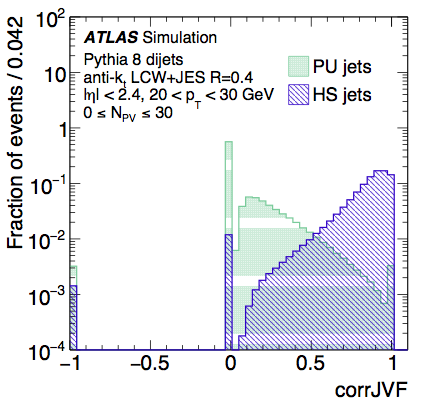
\includegraphics[width=\textwidth]{figures/corrJVF.png}
	\caption{corrJVF}
	\label{fig:corrJVF}
\end{subfigure} % \hspace{0.1\textwidth}
\begin{subfigure}{0.5\textwidth}
   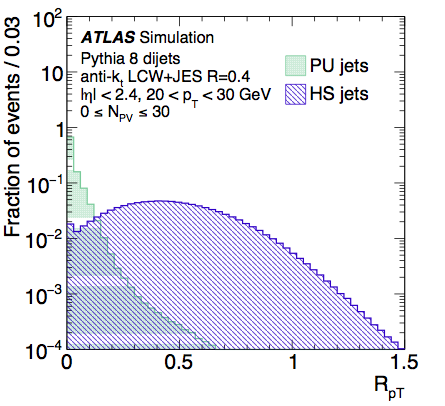
\includegraphics[width=\textwidth]{figures/Rpt.png}
	\caption{$R_{\pt}$}
	\label{fig:Rpt}
\end{subfigure}
\caption{Plots showing distributions of variables used to correct for JVF's dependence on the number of 
reconstructed vertices, and hence number of pileup tracks, in an event. The distributions 
from pileup and hard-scatter jets are overlayed. The simulated jets are reconstructed with the 
LCW scale and the jet energy scale is applied. Taken from Ref~\cite{Aad:2015ina}}
\end{figure}

\par During Run 2 a Jet Vertex Tagger (JVT), which makes use of corrJVF and $R_{\pt}$, 
 is used. corrJVF and $R_{\pt}$ define a 2-dimensional space in which every reconstructed 
jet resides. The k-nearest neighbor (kNN) model~\cite{citeulike:1164920} is used to determine 
the likelihood of a jet to be from hard-scatter (signal) or from pileup (background). This 
model is trained on a sample of signal and background for jets with \pt\ in the range of 
20~\GeV\ and 50~\GeV and $|\eta|<2.4$, where 100 nearest neighbors are used to determine 
the likelihood for a jet to be signal or background. Figure~\ref{fig:jvtROC} shows the fake rate 
from pileup jets versus the efficiency from hard scatter jets from simulation using JVT and other 
discriminants discussed in this section; the JVT curve shows that it is the most optimal of all 
the other pileup suppression techniques. 

\begin{figure}[!h]
\centering
   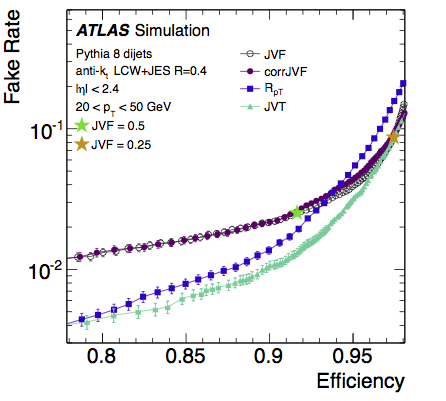
\includegraphics[width=0.8\textwidth]{figures/jvtROC.png}
\caption{Plots showing the fake rate from pileup jets versus efficiency hard scatter jets for JVF, corrJVF, $R_{\pt}$,
and JVT. JVT uses a kNN model in corrJVF-$R_{\pt}$ space where 100 neighbors determine whether a jet is 
from pileup or from hard scatter. Taken from Ref~\cite{Aad:2015ina}}
	\label{fig:jvtROC}
\end{figure}

\par Uncertainties associated with JVF and JVT were calculated by shifting the JVF or JVT selection by 
variations that account for the extent to which the jet correction is mis-modelled for jets 
originating from the primary vertex. These uncertainties vary between 2 and 6\% depending on the 
jet \pt\ and pseudorapidity. 

\subsection{B-Tagging}
\label{sec:bTag}
\par Jets initiated by $b$-quarks are common signatures 
in many processes. For example, in $gg\ra\ttbar$ each 
top quark decays weakly to a bottom quark which then initiates a jet. Several techniques are 
available that tag a jet as $b$-quark initiated. 
$b$-tagging techniques typically exploit the relatively high lifetime 
of the $b$-hadrons, which is of the order of \SI{1.5}{\pico\s}. To put this into perspective, a $b$-hadron 
with $\pt=50~\GeV$ will typically traverse several mm before decaying to $c$-hadrons 
or some other light-flavor hadrons. This section discussed two types of 
$b$-tagging techniques whose details can be found in Ref~\cite{Aad:2015ydr}. 

\par The first technique parameterizes the $b$-hadron lifetime by the impact parameters 
of the tracks in a jet with respect to the primary vertex. The most efficient of algorithms 
that implement this technique is IP3D. It proceeds as follows: For a jet, each track's transverse 
impact parameter with respect to the primary vertex $d_0$ and its longitudinal impact parameter $z_0$
are extracted. A 2-dimensional function of the significance of $d_0$ $(d_0/\sigma(d_0))$, and the 
significance of $z_0$ $(z_0/\sigma(z_0))$ is evaluated and compared to 2-dimensional probability density functions 
for $b$ and light flavor jet hypotheses for each track. These prior probability 
density functions are obtained from Monte Carlo simulations. The ratio of the $b$-jet likelihood to the 
light flavor jet likelihood is taken as the track weight. The weight for the jet is then the 
sum of logarithms of the individual track weights. A simpler version of this algorithm 
is the IP2D, which replaces the 2-dimensional function with a 1-dimensional function of $z_0/\sigma(z_0)$.

\par The second technique constructs a secondary vertex at which the $b$-hadron decays.
The secondary vertex is built by vertices from pairs of tracks with large displacements from the 
primary vertex. These two-track vertices are required to have a fit with a $\chi^2$ lower than a threshold value. 
Additionally, vertices compatible with long lived particles and photon conversions are not considered. 
When building the two-track vertices into the secondary vertex two-track vertices contributing 
the largest $\chi^2$ are removed if the secondary vertex's $\chi^2$ is larger than a threshold value. 
The distance between the primary vertex and the secondary vertex is the discriminant used for 
identifying $b$-jets. One algorithm that implements this technique is called SV1. It uses the 
Log Likelihood Ratio method, where the likelihoods are constructed from two distributions: The 
first is a 2-dimensional distribution of secondary vertex mass versus its energy. The second is 
a 2-dimensional distribution of the number of two-track vertices in the secondary vertex versus 
the $\Delta R$ between the jet axis and the primary-secondary vertices axis.  

\par Another algorithm that constructs a secondary vertex using a slightly different approach is 
called JetFitter. This algorithm runs a trained artificial neural network on 
the jet, looping through each vertex (apart from the primary)
that has at least two tracks. The neural network takes variables that describe the vertex in question 
and has output nodes for either a $b$-vertex or a light flavor vertex. The discriminant to select $b$-jets 
from light flavor jets is taken as the logarithm of the ratio of values in the $b$-node to the value 
in the light flavor node.     

\subsubsection{Performance and Uncertainties}
\par During Run 2 the $b$-tagging algorithms discussed in this section were combined. 
More specifically, in 2015 the combined algorithm was MV2c20 while in 2016 the algorithm used was called MV2c10.
These two algorithms combine IP2D, IP3D, SV1 and JetFitter~\cite{ATL-PHYS-PUB-2016-012}, where 
the variables from each of standalone algorithms were used as inputs to a Boosted Decision Tree (BDT). 
The BDT was trained using jets initiated by $b$-quarks as signal. The background was a composition of 
light-flavor jets, $c$-jets and jets from a hadronic $\tau$ lepton. In MV2c20, 20\% of the background was made up of  
$c$-jets while in MV2c10 10\% of the background was made up of $c$-jets. It was shown that even though MV2c10 
provides similar light-jet rejection to that provided by MV2c20, it provides 40\% more $c$-jet rejection. 
Thus, analyses presented in this text use only MV2c10. Regardless, it is worthwhile to compare 
the performance of MV2c10 against MV2c20.  

\par Figure~\ref{fig:bdtOutput} shows the performance of the MV2c10 BDT output for $b$-, $c$-, and 
light flavor jets in \ttbar\ events. A nominal selection criterion was imposed on the BDT output such that the 
$b$-jet selection efficiency is 77\%. This working point varied with needs. For example, in 
Section~\ref{sec:objCh} the working point was such that the $b$-jet selection efficiency was 70\%. 

\begin{figure}[!h]
\centering
   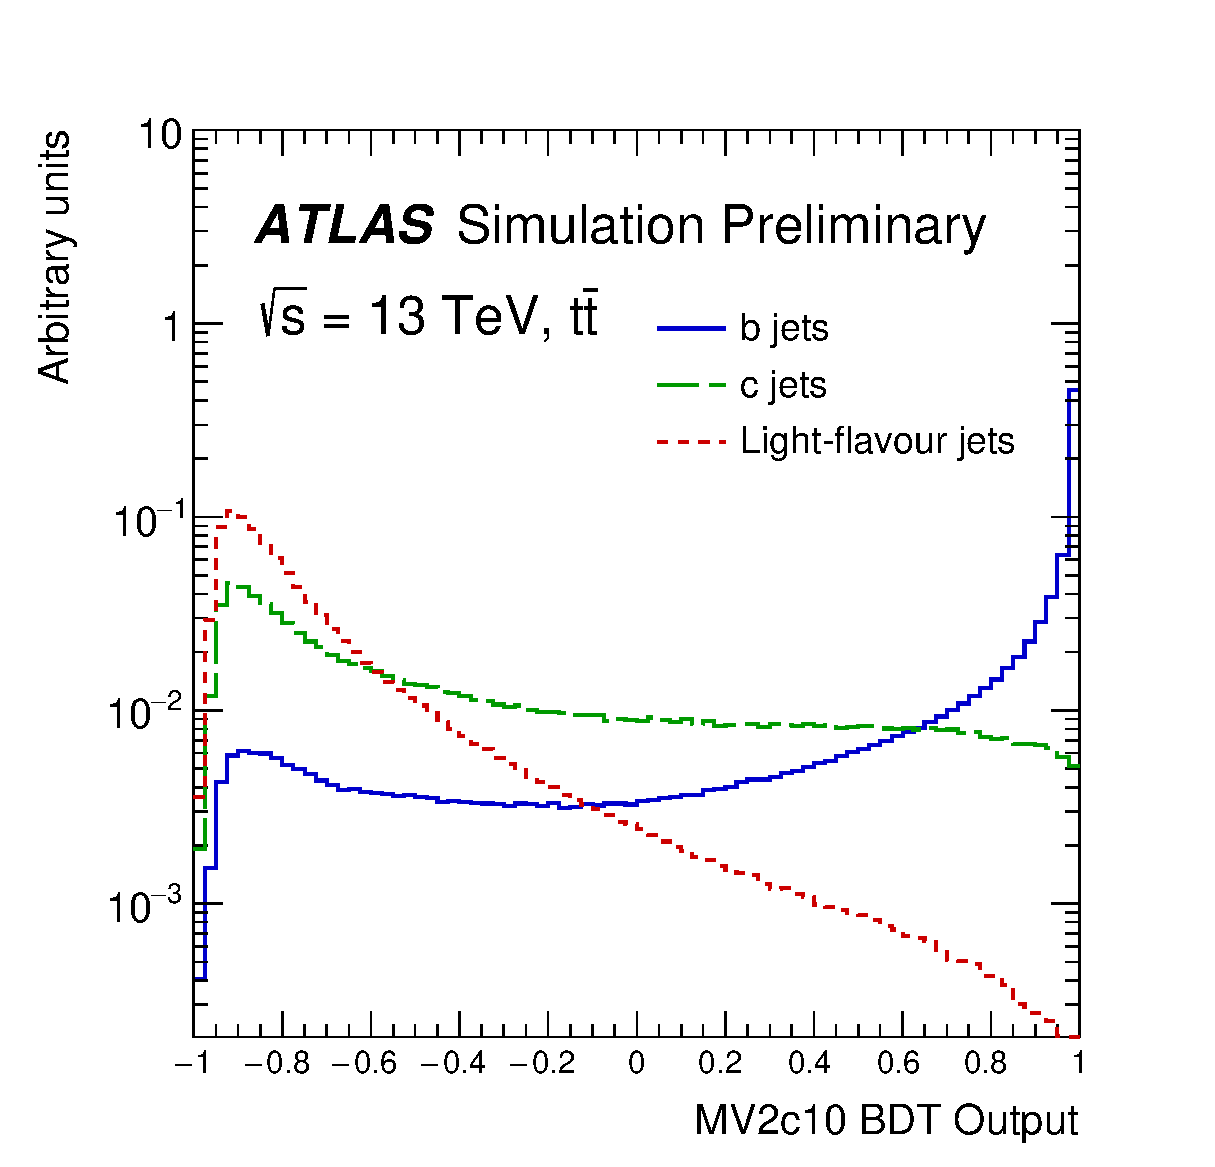
\includegraphics[width=0.8\textwidth]{figures/outputMV2_PRE.eps}
	\caption{Plots showing the MV2c10 BDT output, taken from Ref~~\cite{ATL-PHYS-PUB-2016-012}}
	\label{fig:bdtOutput}
\end{figure}

\par Figure~\ref{fig:effMV2} shows the $b$-jet selection efficiencies, plotted against 
jet \pt, using the BDT outputs from MV2c10 and MV2c20. The working point was 77\% efficiency. 
There is no significant difference between the two algorithms. Figure~\ref{fig:refMV2} shows the 
$c$-jet rejection, plotted against jet \pt, using the BDT outputs from MV2c10 and MV2c20, at a 77\% 
efficiency working point. MV2v10 shows much more improved rejections. That is why it was the 
algorithm of choice in the analysis discussed in Chapter~\ref{chargedH}.   
 
\begin{figure}[!h]
\begin{subfigure}{0.5\textwidth}
   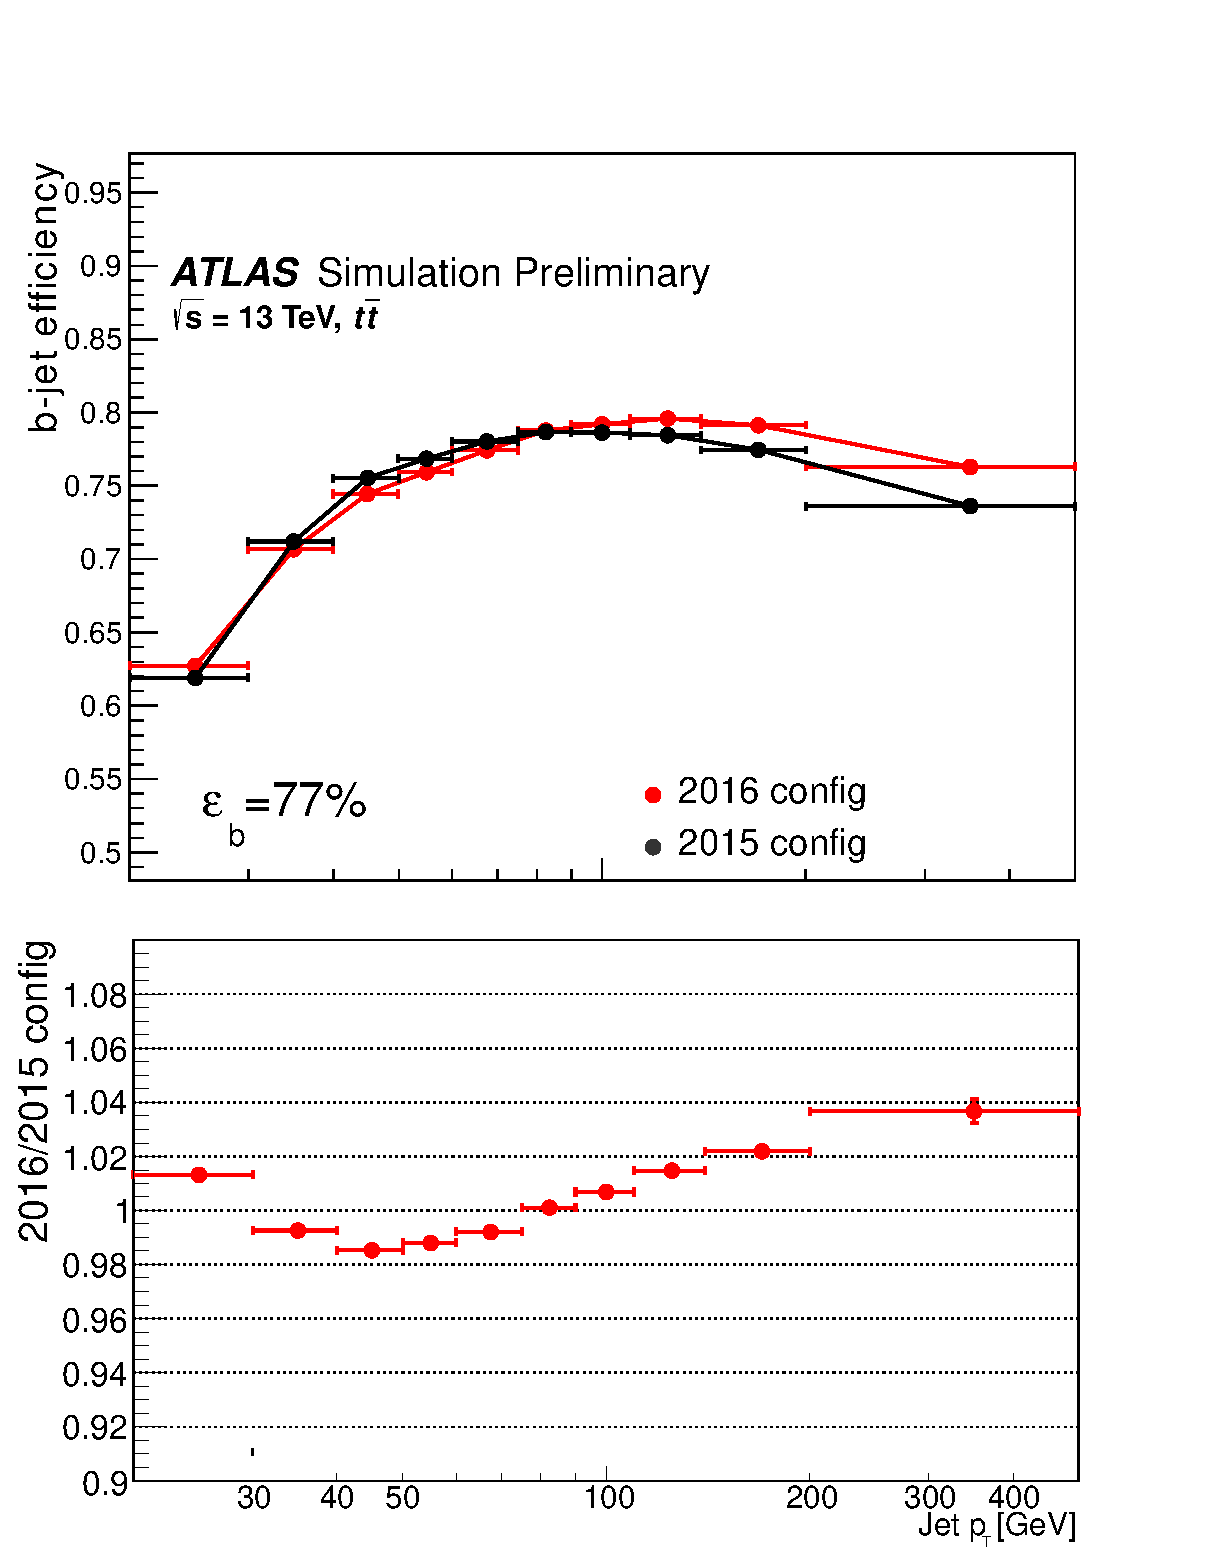
\includegraphics[width=\textwidth]{figures/efficiencyA_PREbis.eps}
	\caption{$b$-jet efficiency}
	\label{fig:effMV2}
\end{subfigure} % \hspace{0.2\textwidth}
\begin{subfigure}{0.5\textwidth}
   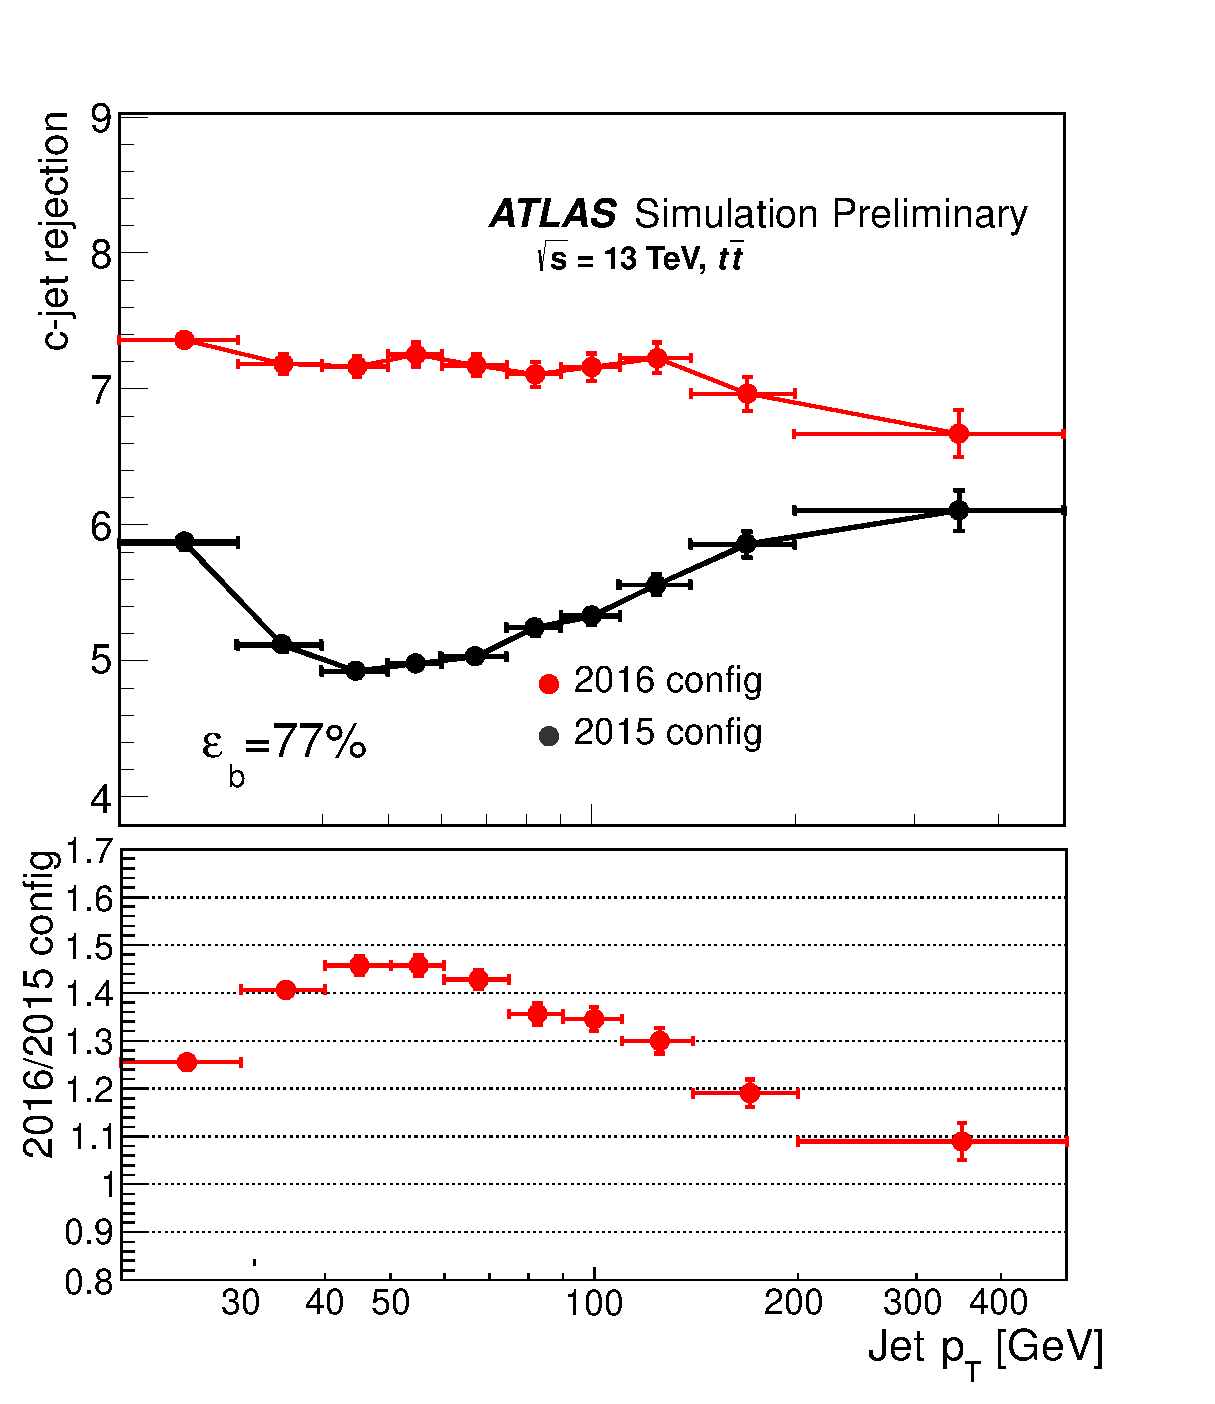
\includegraphics[width=\textwidth]{figures/bc0_modified4BIS_PRE.eps}
	\caption{$c$-jet rejection}
	\label{fig:refMV2}
\end{subfigure}
	\caption{Plots showing the $b$-jet efficiency and $c$-jet rejection parametrized with jet \pt, for the MV2c10 (2016 config)
and the MV2c20 (2015 config) algorithms, at a 77\% $b$-jet selection efficiency working 
point. Taken from Ref~~\cite{ATL-PHYS-PUB-2016-012}}
\end{figure}

\par $b$-tagging efficiencies in Monte Carlo simulations were corrected to match efficiencies obtained in 
regions in data rich in the physics processes modelled by the said Monte Carlo simulations. Uncertainties on the 
$b$-tagging efficiencies were evaluated by shifting the BDT output value by an up and a down value, and 
evaluating the impact on the physics process prediction. More analysis-specific details on this in 
Section~\ref{sec:objCh}. 


	\section{Taus}
	\label{sec:tau}
\par As discussed in Section~\ref{sec:sm}, of all leptons the $\tau$ lepton has the smallest 
mean lifetime of \SI{2.9e-13}{\s} ($c\tau \approx \SI{87}{\micron}$), 
decaying inside the LHC beam pipe.\footnote{The LHC beam pipe has 
an external diameter of about 5.3~cm.}
Also the heaviest of all the leptons, the $\tau$ lepton is the only lepton 
heavy enough to decay to hadrons, with a branching ratio of approximately 
65\%. The said hadrons are dominated by neutral and charged pions, although 2.7\% of the 
time the $\tau$ lepton decays to kaons. 

\subsection{Reconstruction and Identification}
\par When a $\tau$ lepton decays hadronically it is referred to 
as a hadronic $\tau$, otherwise it is reconstructed as the electron or muon that 
it decays to (See Sections~\ref{sec:ele} and \ref{sec:mu}). In either case, there is a $\nu_\tau$
in the final decay products. Since this $\nu_\tau$ is invisible in the ATLAS detector the hadronic $\tau$ 
is reconstructed through its visible decay products, which are referred to as $\tauvis$.
As discussed in Section~\ref{sec:sm} the $\tau$ lepton is restricted to decaying to an 
odd number of charged mesons, with decreasing branching ratios as the odd number increases. 
In ATLAS the most common hadronic $\tau$ decays constitute 1 or 3 charged pions, sometimes with associated 
neutral pions. 

\subsubsection{Reconstruction}
\par The $\tauvis$ signature in ATLAS comprises some energy deposits in the 
calorimeters, matched to 1 or 3 ID tracks.\footnote{$\geq$5 ID tracks are very rare.} 
$\tauvis$ with 1 matched track are 
called {\it 1-prong}, and those with 3 matched tracks are called {\it 3-prong}. 
Since neutral pions decay as $\pizero\to\gamma\gamma$, a significant component of the energy is deposited in 
the electromagnetic calorimeters for those $\tau$ lepton decays that include neutral pions. 

\par The largest background to the hadronic $\tau$ 
is the QCD jet, although electrons and muons can be reconstructed as $\tauvis$ as well. 
With a smaller transverse mass, $\tauvis$ components from a hadronic $\tau$ tend to be more 
collimated than those from a QCD jet for a given $\pt$. Moreover, due to higher particle 
multiplicity in a QCD jet, a QCD jet tends to have a higher ID track multiplicity  
than a hadronic $\tau$ for a given $\pt$. These two differences are used to reduce the QCD jet 
background contamination, as discussed in Section~\ref{sec:idTauJets}.
     
\par Topological clusters in all jets with $\pt>10~\GeV$ and $|\eta|<2.5$, reconstructed as discussed in Section~\ref{sec:jets},
 are used as seeds by the $\tau$ reconstruction algorithm. Tracks from the ID that satisfy a 
the selection criteria shown in Table~\ref{tab:tautrkSel} are matched to the $\tauvis$ candidate,  
using the center of the vector sum of all the topological 
clusters (henceforth known as the $\tauvis$ center) as reference. This reference point 
may not be the same as the center of the reconstructed jet 
because the jet center undergoes corrections described in Section~\ref{sec:jetCalib}.
Tracks from the ID that lie within $\Delta R<0.2$ around the $\tauvis$ center are counted 
as tracks from the $\tau$ decay. The $\tau$ candidate is then classified as either 1-prong 
or 3-prong, depending on the number of tracks found within $\Delta R<0.2$. 
Energy from topological clusters that lie within $\Delta R<0.2$ around the $\tauvis$ center are summed up to compute the 
total transverse energy $\eT$ of the $\tauvis$ candidate, which is taken as equal to $\pT$, on account 
of the small $\tau$ lepton mass. The 
$\tauvis$ is then characterized by $\pt,\eta$ and $\phi$, where $\eta,\phi$ are 
the $\tauvis$ center coordinates. 
Further, the following regions in relation to the $\tauvis$ center are defined:

\begin{enumerate}
\item $\Delta R<0.1$, as the {\it calo-core} region;
\item $\Delta R<0.2$, as the {\it core} region;
\item and $0.2<\Delta R<0.4$, as the {\it isolation ring}.
\end{enumerate} 

\begin{table}[!h]
\centering
   \begin{tabular}{|c|}
\hline
{\bf Selection Criteria} \\
\hline\hline \\
$\pt>1~\GeV$ \\
Number of b-Layer hits $\geq 1$ \\
Number of Pixel Detector hits $\geq 2$ \\
Number of Silicon Detector hits $\geq 7$ \\
$|d_0|<1.0$ mm \\
$|z_0\sin\theta|< 1.5$ mm \\ 
\hline
   \end{tabular}
\caption{Selection criteria for tracks from the Inner Detector that are matched to $\tau$-jet candidates.}
\label{tab:tautrkSel}
\end{table}

\subsubsection{Identification against QCD Jets}
\label{sec:idTauJets}
\par To further reduce the fraction of QCD jets that are reconstructed as $\tauvis$, a separate 
identification algorithm is applied on the reconstructed hadronic $\tau$ lepton. Several variables,
 designed to exploit the differences in shower width and track multiplicity between 
hadronic $\tau$ jets and QCD jets, are used. Only a few are discussed here, but for a more detailed discussion the reader should 
consult Ref~\cite{ATLAS:tauvars}. 

\begin{enumerate}
\item 
\begin{equation*}
f_{\text{core}} = \frac{\sum_{i\in\text{calo-core}} E_{T,i}^{EM}}{ \sum_{j}^{\Delta R_i\in\text{core}} E_{T,j}^{EM}}
\end{equation*}
is the fraction of transverse energy deposited in topological clusters in the core-calo region, to that deposited in the core
 region. The energy deposits are calibrated at the EM scale. For studies used in this analysis, 
a more pile-up robust version of this variable is $f_{\text{core}}^{\text{corr}}$ used, 
after correcting for pile-up events by taking into account the number of vertices with at least 2 tracks in the event.  

\item 
\begin{equation*}
f_{\text{track}} = \frac{\pT^{\text{leadTrk}}}{ \sum_{j\in\text{core}} E_{T,j}^{EM}}
\end{equation*}
is the ratio of the transverse momentum of the track with the highest transverse momentum, to energy deposits in the core 
region of the $\tauvis$. Here, a pile-up corrected version $f_{\text{track}}^{\text{corr}}$ is used, just like in the 
$f_{\text{core}}$ case. 

\item 
\begin{equation*}
R_{\text{track}} = \frac{\sum_i^{\Delta R_i<0.4}(\pti\times\Delta R_i)}{\sum_i^{\Delta R_i<0.4} \pti} 
\end{equation*}
is the transverse radius defined by the $\tauvis$ tracks, weighted by the \pt\ of the tracks. 

%\item 
%\begin{equation*}
%R_{had} = \frac{\sum_{i\in\{Had\}}^{\Delta R_i<0.4} (E_{T,i}\times\Delta R_i)}{ \sum_{i\in\{Had\}}^{\Delta R_i<0.4} E_{T,i}}
%\end{equation*}
% is  
%defined as the $\tauvis$ transverse radius in the hadronic component of the calorimeter. It is a ratio of the 
%distance-weighted sum of hadronic topoclusters energies to their unweighted sum. The expectation is that $\tau$ leptons would 
%generally have a smaller $R_{had}$ than QCD jets.  
%
%\item 
%\begin{equation*}
%R_{cal} = \frac{\sum_{i\in\{EM\}}^{\Delta R_i<0.4} (E_{T,i}\times\Delta R_i)  + \sum_{i\in\{Had\}}^{\Delta R_i<0.4} (E_{T,i}\times\Delta R_i) }{ \sum_{i\in\{EM\}}^{\Delta R_i<0.4} E_{T,i} + \sum_{i\in\{Had\}}^{\Delta R_i<0.4} E_{T,i} }
%\end{equation*}
% is defined 
%as the $\tauvis$ transverse radius in all calorimeter components. 
%It is similar to $R_{had}$, differing in that it includes topoclusters from the electromagnetic calorimeters. 
%$R_{cal}$'s expectations are similar to those of $R_{had}$.
%
\end{enumerate}

\par Some variables were showed stronger discrimination strength when applied either to 1-prong 
or 3-prong $\tauvis$. For example, for 1-prong $\tauvis$ candidates the impact parameter 
significance ($d_0/\delta d_0)$ of the track  with the highest \pT, and the number of tracks in the 
isolation ring are used. For 3-prong $\tauvis$ candidates the maximal $\Delta R$ between the $\tauvis$
tracks and its center, and the invariant mass of the track system are used. 

\par With these and other variables each $\tauvis$ candidate lies in a multivariate hyper-space. Monte-Carlo 
simulations are used to train Boosted Decision Trees (BDTs).
\Ztautau\ and \Wtaunu\ events from simulated samples are used as signal to train the 
BDT on $\tau$ leptons while QCD multi-jets from data are used to train the BDT on QCD jets. 
The BDT is trained in several distinct categories to maximize its classification 
strength. The first categorization is $n$-prong, separating the candidates according to their 
associated tracks.
The second categorization is the reconstructed $\tau$ \pt. The \pt\ ranges are 
0$\to$45~\GeV, 45$\to$100~\GeV, and 100$\to\infty$~\GeV. The last categorization is the number of 
vertices in the event, to get a handle on pileup effects. The number of vertices are 
categorized into ranges of 1$\to$3, 4$\to$7, and 8$\to\infty$.   

\par There are three working points for $\tau$ identification. {\it Loose} is defined at a target signal 
selection efficiency of 70\% for 1-prong and 65\% for 3-prong $\tauvis$. Likewise, the {\it medium} 
working point targets a signal efficiency of 60\% for 1-prong and 55\% for 3-prong $\tauvis$. Lastly, 
the {\it tight} working point targets a signal efficiency of 40\% for 1-prong and 35\% for 3-prong.  
%Figure~\ref{fig:tauEff} shows identification efficiencies of signal and background as a function of 
%$\pt$ and the number of vertices, categorized into the number of prongs. 
%
%\begin{figure}[h]
%%   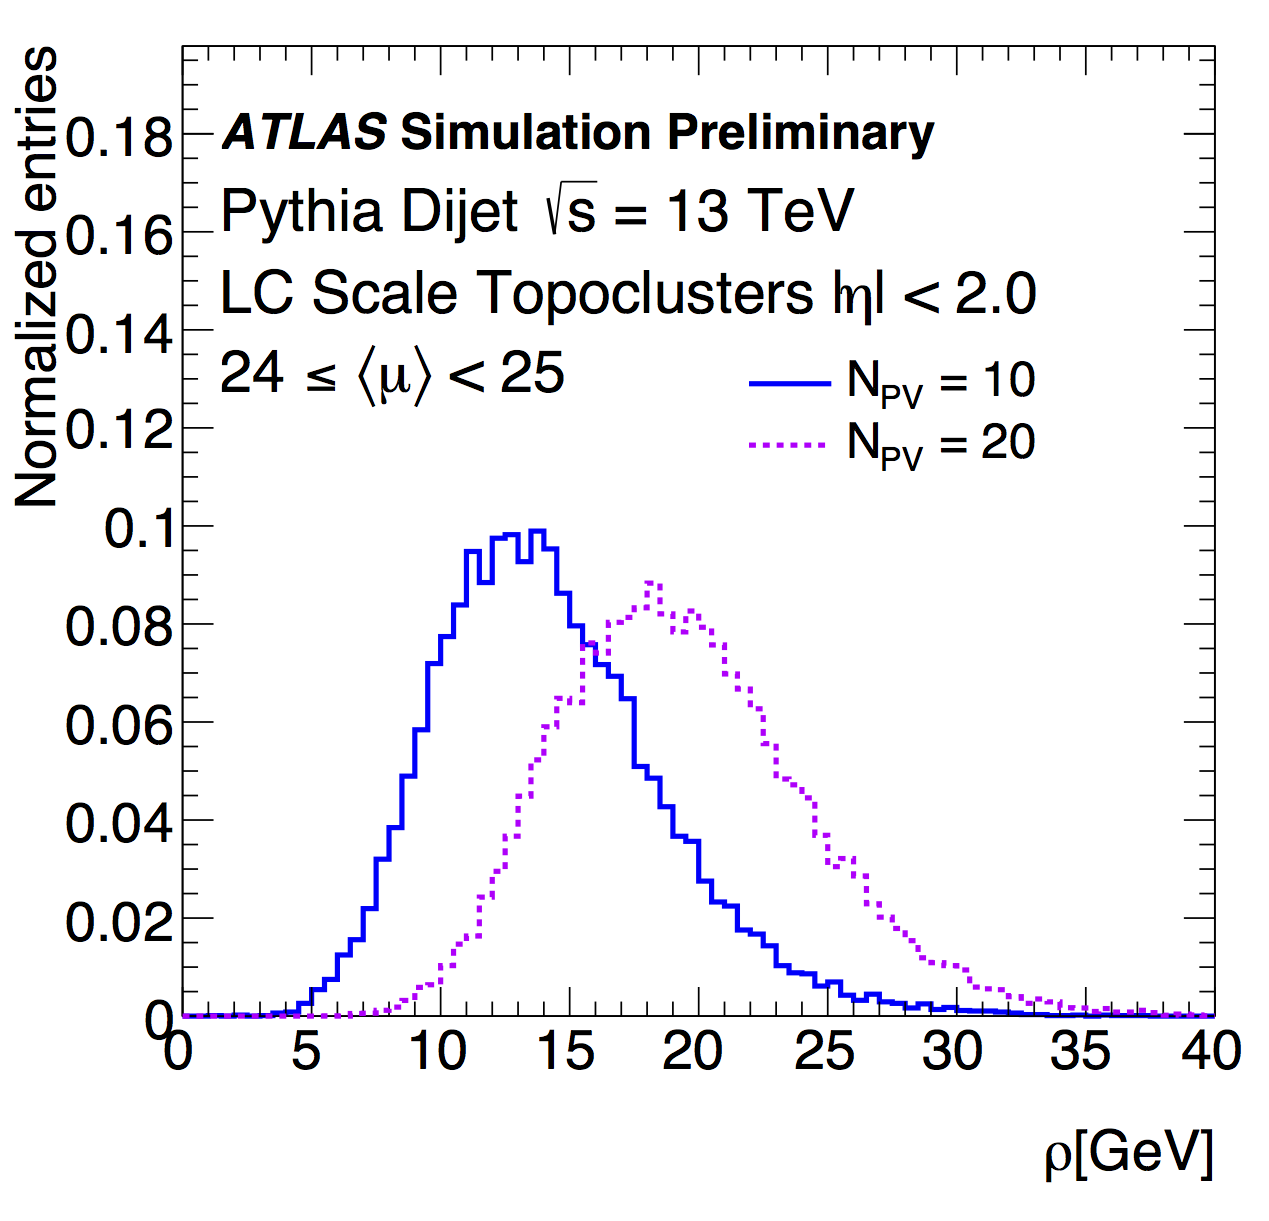
\includegraphics[width=\textwidth]{figures/rho13.png}
%\rectangle{\linewidth}{0.5cm}
%	\caption{Identification efficiency distributions for hadronic $\tau$ leptons and for QCD jets (background)} 
%	\label{fig:tauEff}
%\end{figure}

\subsubsection{Identification against electrons and muons}
\par As already hinted, electrons and muons may also be reconstructed as hadronic $\tau$ leptons. 
This is more common for electrons than it is for muons because muons rarely deposit most of their 
energy in the calorimeters. Since an electron is likely to be associated with one track, 1-prong 
$\tauvis$ suffer a lot more electron contamination than 3-prong electrons. 

\par A BDT is used to train hadronic $\tau$ signal and electron backgrounds. Monte Carlo simulation samples of 
$\Ztautau$ and $\Zee$ are used for these respective tasks. Both the electron and $\tau$ candidates 
are required to pass $\pT>20~\GeV$. The $\tauvis$ is further required to pass the BDT loose 
selection criteria. Upon overlap between and electron and a $\tauvis$, an electron is preferred.    
The BDT was trained in categories of $|\eta|<1.37, 1.37<|\eta|<2.0, 2.0<|\eta|<2.3$ and 
$|\eta|>2.3$.

\par Apart from $f_{\text{core}}^{\text{corr}}, f_{\text{track}}^{\text{corr}}$ and $R_{\text{track}}$
 some variables that enhanced electron/$\tau$ separation were used. These are 
\begin{enumerate}
\item 
\begin{equation*}
f_{iso} = \frac{\sum_{i\in\text{isolation ring}}E_{T,i}^{EM}}{\sum_{j}^{\Delta R<0.4} E_{T,j}^{EM}},
\end{equation*}
compares the width of the electron and $\tauvis$ showers. Although the electron shower is not expected 
to be much wider than the $\tauvis$ shower, some differences at the core level are expected;

\item and $f_{\text{HT}}$, the ratio of high-threshold to low-threshold hits in the TRT. Electrons, being 
lighter than pions (from the $\tau$ decay), have higher Lorentz factors ($\gamma$). So they are 
expected to produce more high-threshold hits in the TRT than hadronic $\tau$ leptons.  
\end{enumerate} 

%\par Figure~\ref{fig:eleTauEff} shows identification efficiencies of signal and background, 
%categorized in $\eta$. 
%
%\begin{figure}[h]
%%   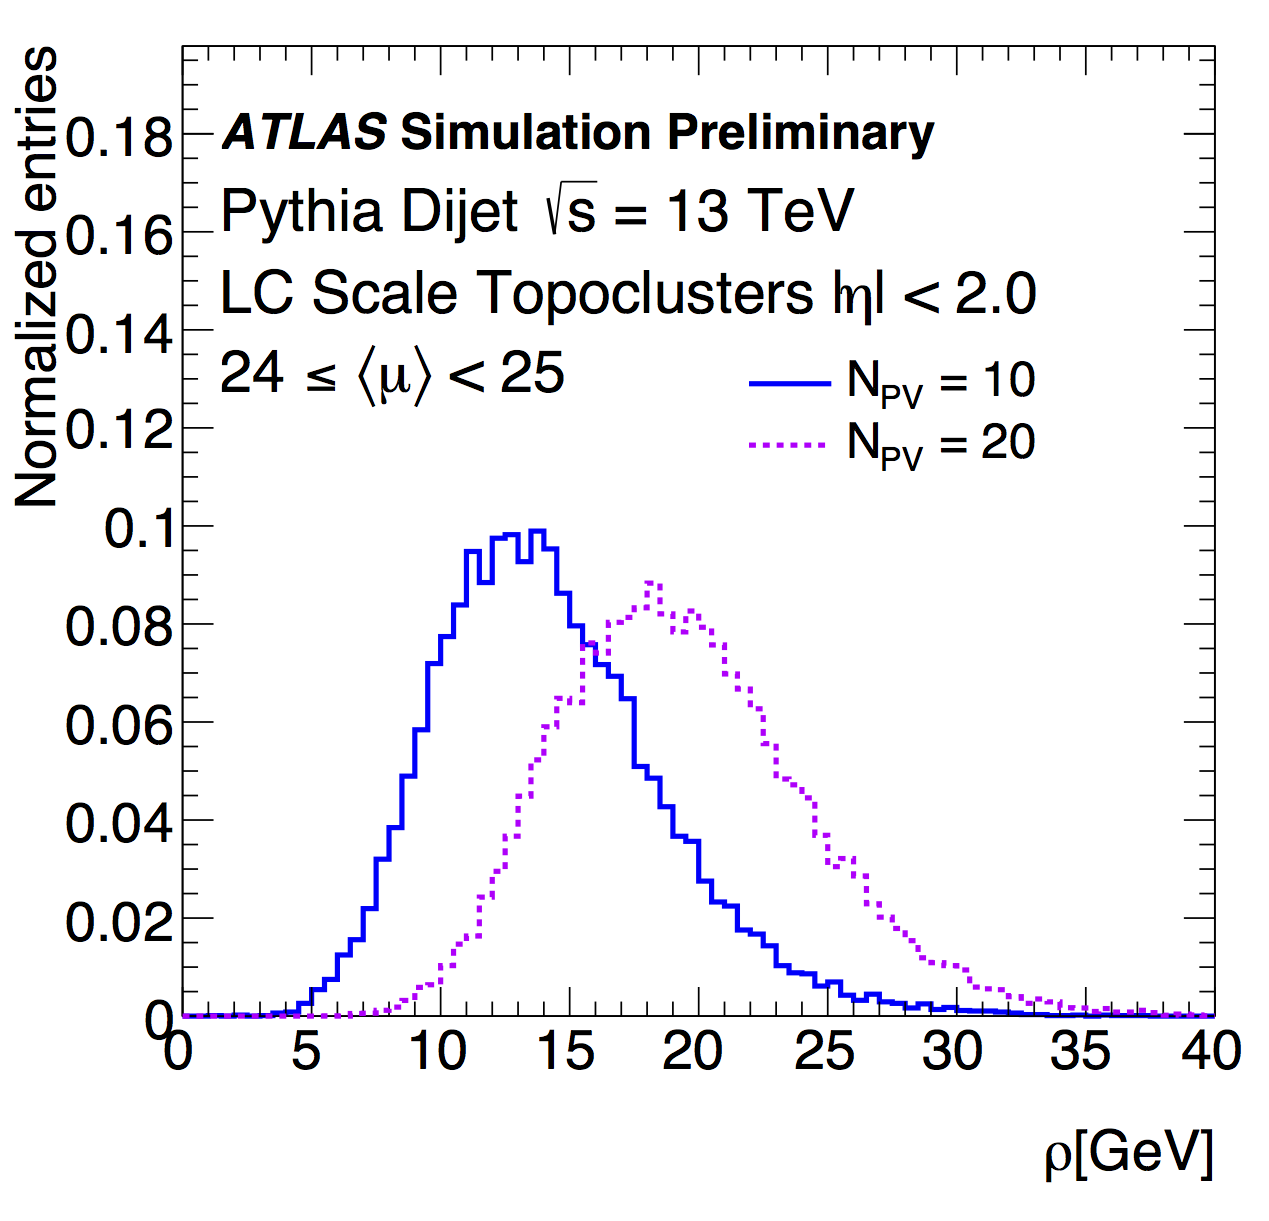
\includegraphics[width=\textwidth]{figures/rho13.png}
%\rectangle{\linewidth}{0.5cm}
%	\caption{Identification efficiency distributions for hadronic $\tau$ leptons and for electrons (background)} 
%	\label{fig:eleTauEff}
%\end{figure}
%
%\par Muons ...
%****
%muons
%****
% 1. only two variables used ... fTrack and fEM
% 2. In my code no scale factors seem to be applied though ... Confused.
%
%\subsubsection{Identification Efficiency}
%TO DO ... Describe in detail how identification efficiencies for MC are extracted and applied
% 1. objective is to calculate eff in data, and in sim and obtain scale factors
% 2. eff in sim is trivial because the tauvis is matched to truth
% 3. eff in data is obtained in a dedicated region
% 4. this region in practice has backgrounds. they need to be quantified
% 5. choose a variable that's good at separating background and signal (extended Ntracks)
% 6. get predictions of variable for expected signal, background and fit to data
% 7. perform fit before and after ID, as they change

% 1. Ztautau events
% 2. Wtau
% 3. ttbar 


%\subsection{Systematic Uncertainties}


	\section{Missing Energy}
	\label{sec:met}
\par The longitudinal momentum of the proton constituents during $pp$ collisions at the LHC 
is not known. Rather, the total transverse momentum of these constituents is expected to be 
insignificantly smaller than the longitudinal momentum. So, the total transverse momentum 
before a $pp$ collision can be taken as zero. Due to conservation of momentum, it should also 
be zero after the collision. In other words, transverse momentum imbalance, also known 
as {\it missing transverse energy (MET, or $\boldsymbol{\met}$)}, is expected to be zero if all decay products were 
detectable by the ATLAS detector.  

\par Neutrinos leave no signature in the ATLAS detector; they are invisible. 
Their presence is inferred by the presence of $\boldsymbol{\met}$, whose $x$ and $y$ components 
are defined as 

\begin{dmath}
E^{\text{miss}}_{x(y)} = E^{\text{miss},e}_{x(y)} + E^{\text{miss},\gamma}_{x(y)} +E^{\text{miss},\tau}_{x(y)} +E^{\text{miss,jets}}_{x(y)} + E^{\text{miss},\mu}_{x(y)} + E^{\text{miss,soft}}_{x(y)}, 
\label{eq:metDef}
\end{dmath} 

where each term is either the negative sum of \pt components, or the negative sum of cell energies, weighted according to their position in $\eta$ and $\phi$ as follows : 

\begin{equation}
\begin{aligned}
E^{\text{miss,term}}_{x} = \sum_{i=1}^{N^{\text{term}}_{\text{cell}}}E_i\sin\theta_i\cos\phi_i  & \text{ and} & 
E^{\text{miss,term}}_{y} = \sum_{i=1}^{N^{\text{term}}_{\text{cell}}}E_i\sin\theta_i\sin\phi_i.  
\end{aligned}
\end{equation}

The $E^{\text{miss,soft}}_{x(y)}$ term is called the {\it soft term}, and the sum of the other terms is collectively called 
the {\it hard term}. Reconstruction of the soft and hard terms differs slightly between 
Run I and Run II, as discussed in Sections~\ref{sec:runImet} and~\ref{sec:runIImet}.
To avoid ambiguities in the detector signals used to construct the physics objects used in the hard term, 
a priority list is defined. Electrons, having the highest purity, are considered first, followed by 
photons, hadronic $\tau$ leptons, muons and finally jets. This means that objects low in the 
priority list are removed from the list if they share detector signals with objects higher in the 
priority list.  

\par Approximating the neutrino masses with zero, $\boldsymbol{\met}=\boldsymbol{p_{\mathrm T}^{\mathrm{miss}}}$. These 
two quantities are therefore used interchangeably in this text.  

\par The magnitude of $\boldsymbol{\met}$ is then   

\begin{equation}
\met = \sqrt{(E^{\text{miss}}_x)^2 + (E^{\text{miss}}_y)^2}
\end{equation}
 
and its $\phi$ direction is 

\begin{equation}
\phi^{\text{miss}} = \arctan(E^{\text{miss}}_y,E^{\text{miss}}_x).
\end{equation}   

The scalar sum of the \pt\ of all the objects in the event is then 

\begin{equation}
\sum\eT = \sum_{i\in\text{hard}}p_{\text{T,i}} + \sum_{j\in\text{soft}}p_{T,j}.
\end{equation}

\subsection{Run I Reconstruction}
\label{sec:runImet}
\par While the hard term in Run I reconstruction is formulated as in Equation~\ref{eq:metDef}, the soft term is formulated as 
 
\begin{dmath}
E^{\text{miss,soft}}_{x(y)} = E^{\text{miss,softjets}}_{x(y)} +E^{\text{miss,CellOut}}_{x(y)} + (E^{\text{miss,calo},\mu}_{x(y)}),
\label{eq:softmetDef}
\end{dmath} 

where the parentheses on one of the terms hint towards a caveat. 

\par $E^{\text{miss},e}_{x(y)}, E^{\text{miss},\gamma}_{x(y)}$ and $E^{\text{miss},\tau}_{x(y)}$ are calculated from cells in clusters 
associated with electrons, photons and hadronic $\tau$ leptons respectively. The electrons and photons are calibrated at the 
electromagnetic scale, while the hadronic $\tau$ leptons are calibrated with the LCW scheme. 
Electrons, photons and hadronic $\tau$ leptons used for this calculation are required to have at least 10~\GeV\ in \pt.
While electrons are required to pass the medium identification criteria, photons and hadronic $\tau$ leptons are 
required to pass the tight identification criteria. While both $E^{\text{miss,softjets}}_{x(y)}$ and  
$E^{\text{miss,jets}}_{x(y)}$ use LCW-calibrated jets reconstructed as in Section~\ref{sec:jets}, the former uses 
jets with $7<\pt<20~\GeV$ and the latter uses jets with $\pt>20~\GeV$. Calorimeter cells 
not associated to any reconstructed object are calibrated using the LCW scheme and used to reconstruct 
 $E^{\text{miss,CellOut}}_{x(y)}$. 

\par And now the $E^{\text{miss,calo},\mu}_{x(y)}$ caveat: When a muon is isolated from calorimeter jets, 
as determined by $\Delta R=0.3$, $E^{\text{miss},\mu}_{x(y)}$ is reconstructed from the muon \pt\ 
measured in the Muon Spectrometer and corrected for the energy lost in the calorimeters. In this case, 
 $E^{\text{miss,calo},\mu}_{x(y)}$ is not used in Equation~\ref{eq:metDef}. Otherwise, 
$E^{\text{miss},\mu}_{x(y)}$ is reconstructed from the muon \pt\ measured in the Muon Spectrometer 
and $E^{\text{miss,calo},\mu}_{x(y)}$ is not used in Equation~\ref{eq:metDef}.

\par The object selection criteria used to construct \met\ described in this section is constant. This 
means that \met\ is constant for each event, even if the physics objects in that event are selected with 
a different criteria.
 
\subsubsection{Performance and Uncertainties}
\par Performance of this \met\ reconstruction scheme was tested in $W\to l\nu$, $Z\to ll$ and events 
with only two jets. Performance in data was compared to expected perfomance in Monte Carlo simulation. 
In $W\to l\nu$ events the \met\ is expected to be reconstructed from the neutrino. In $Z\to ll$ no \met\ 
is expected, except from imperfections in the reconstruction scheme. Figures~\ref{fig:metPerfA} and 
\ref{fig:metPerfB} show \met\ 
distributions in regions in data rich in $Z\to ll$ and $W\to l\nu$ respectively.

\begin{figure}[!h]
\begin{subfigure}{0.5\textwidth}
   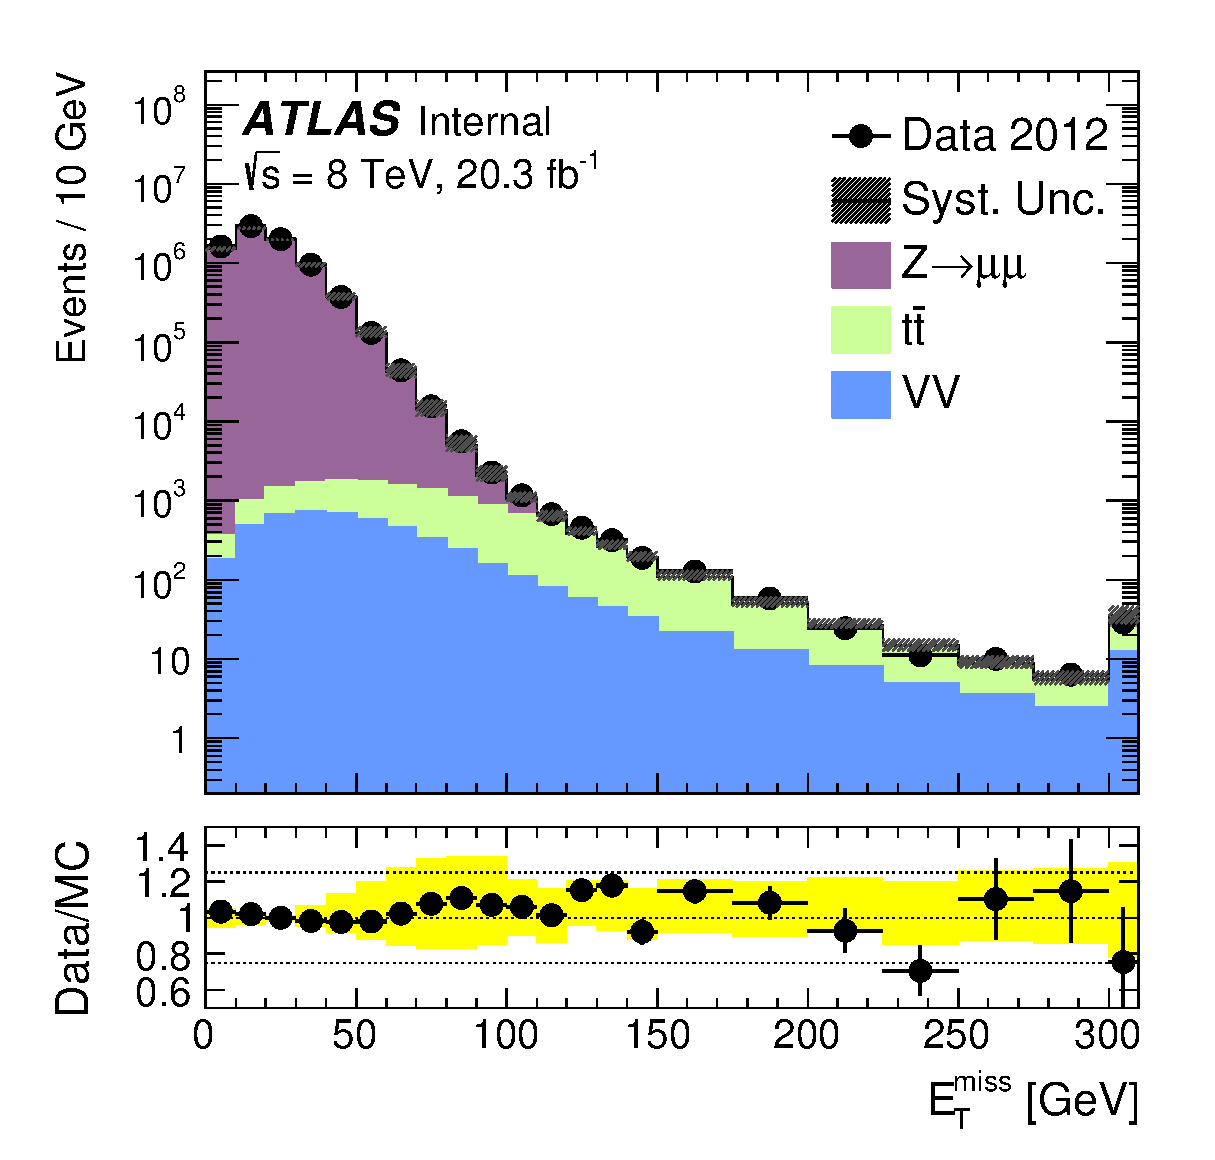
\includegraphics[width=\textwidth]{figures/zmmh_tot_MET.eps}
\caption{\met\ in a $Z\to ll$-rich region in data}
\label{fig:metPerfA}
\end{subfigure} % 
\begin{subfigure}{0.5\textwidth}
   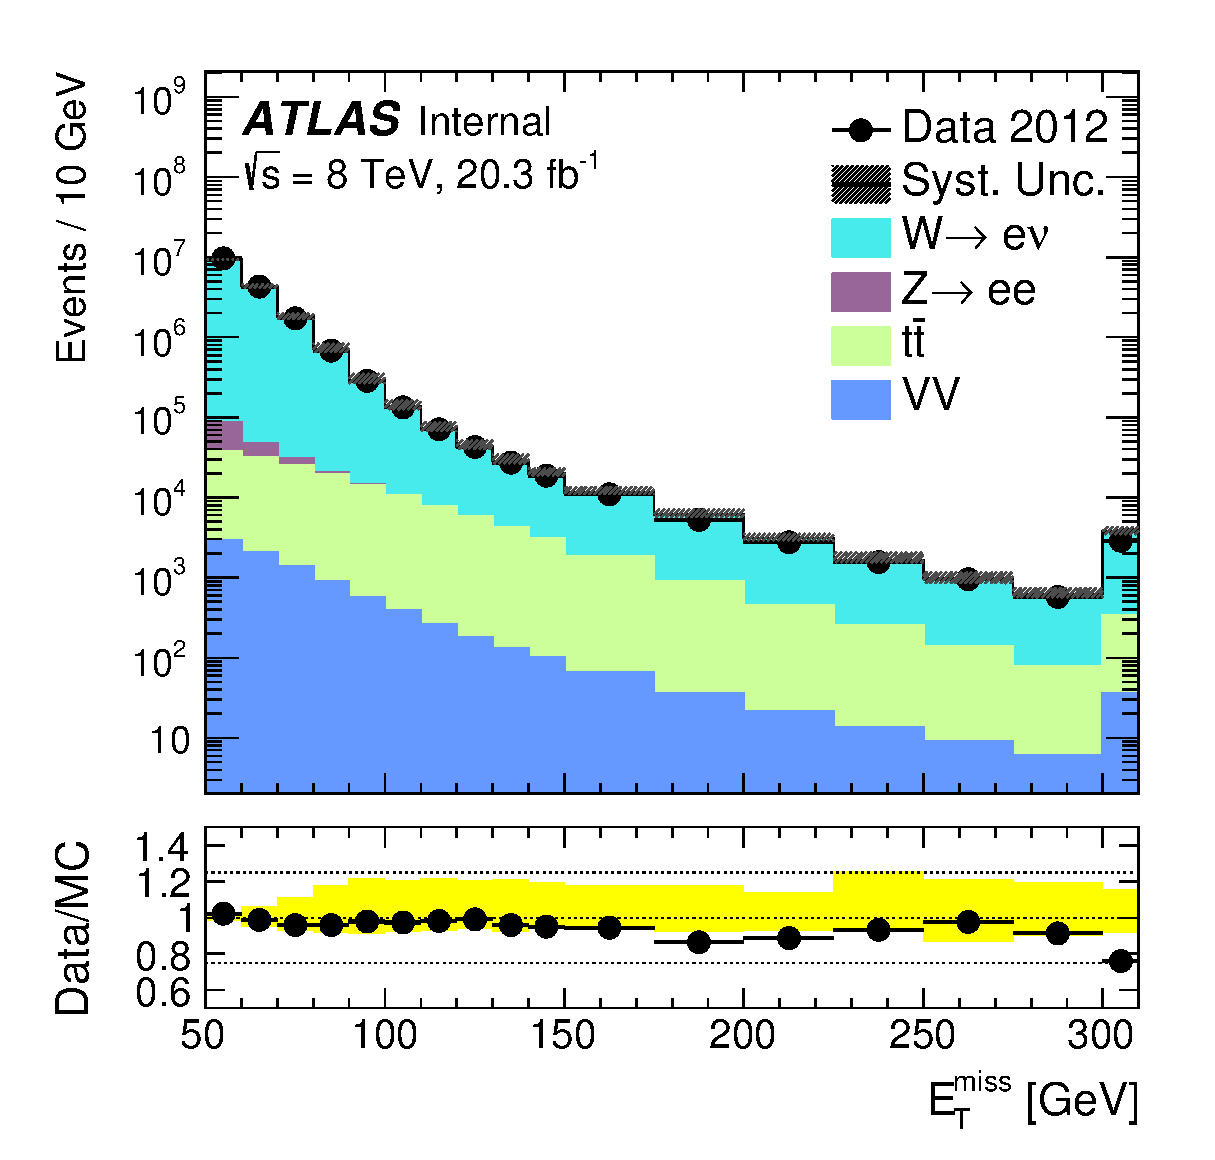
\includegraphics[width=\textwidth]{figures/wenh_tot_MET.eps}
\caption{\met\ in a $W\to l\nu$-rich region in data}
\label{fig:metPerfB}
\end{subfigure}
\caption{Plots showing distributions of \met\ in data, compared to predictions from Monte Carlo distributions, taken from 
Ref~\cite{Khoo:2012749}}
\end{figure}

\par To quantify the \met\ 
performance, its resolution was approximated by the standard deviations 
$\sigma(E^{\text{miss}}_{x(y)} - E^{\text{miss,true}}_{x(y)})$ as functions of $\sum \eT$. 
Since no \met\ was expected in $Z\to ll$ events, these standard deviations were reduced 
to $\sigma(E^{\text{miss}}_{x(y)})$. In $W\to l\nu$ events $E^{\text{miss,true}}_{x(y)})$ 
was obtained from Monte Carlo simulation, so resolutions were studied only in simulation. Contrastingly, in $Z\to ll$ 
events resolutions in data and in Monte Carlo simulation were compared. Either way, these resolutions were observed 
to fall between 5 and 30~\GeV, worsening with increasing $\sum \eT$.

\par Uncertaintiy in the \met\ scale was propagated from the scale uncertainties in the 
individual terms. The uncertainties in the electron, muon, jets, and hadronic $\tau$ terms 
were obtained by methods described in Sections~\ref{sec:ele},~\ref{sec:mu},~\ref{sec:jets}, and 
\ref{sec:tau}. The scale uncertainties in the $E^{\text{miss,softjets}}_{x(y)}$ and $E^{\text{miss,CellOut}}_{x(y)}$ 
terms, collectively known as {\it soft terms}, were evaluated by varying energy 
scales in the topological clusters that contributed to those terms in Monte Carlo 
simulation. After the scale uncertainties from all terms in Equation~\ref{eq:metDef} were evaluated, 
the overall scale uncertainty on \met\ using $W\to l\nu$ Monte Carlo events was found to be 
about 2.6\%. 

\subsection{Run II Reconstruction}
\label{sec:runIImet}
\par The hard terms during Run II reconstruction are formulated just like in Equation~\ref{eq:metDef}.
The selection criteria for the physics objects is however not constant, and consequently \met\ varies 
with the physics object selection. The Run II \met\ used in this thesis is further discussed in 
Section~\ref{sec:objCh}.  

\par To evaluate the perfomance of this reconstruction method a base physics object selection was used. 
The calibration schemes for each of these objects was identical to those used during Run I reconstruction.
Electrons, photons and hadronic $\tau$ leptons were required to not fall in the 
transition region between the central and end-cap calorimeters. 
Electrons were required to be pass the medium selection criteria and have $\pt>10~\GeV$. 
Photons were required to be tightly identified, have $\pt>25~\GeV$. Hadronic $\tau$ leptons 
were required to be of medium quality and have $\pt>20~\GeV$. Muons were required to be of medium 
quality, fall in $|\eta|<2.7$ and have $\pt>10~\GeV$. All jets used had $\pt>20~\GeV$ and $|\eta|>2.4$, or 
$\pt>50~\GeV$ and $|\eta|<4.5$. Any jets with $20<\pt<50~\GeV$ and $|\eta|<2.4$ were required to pass 
additional selection criteria, discussed in Ref~\cite{Brunt:2149445}; other criteria to 
resolve overlaps between objects are also discussed in the same Ref.  

\par The soft term was reconstructed from the \pt\ of tracks in the Inner Detector not associated to any of the 
physics objects discussed in the preceding paragraph. These tracks were required to have at least 
400~\MeV\ in \pt\ and satisfy all track quality criteria discussed in Section~\ref{sec:tracking}.   
In addition, these tracks were required to originate from the primary vertex. This additional requirement 
enabled the soft term to be pileup-robust. 

\subsubsection{Performance and Uncertainties}
\par Performance of \met\ was tested in $Z\to ll$ and $W\to l\nu$ events, just like during 
Run I. Figures~\ref{fig:metPerfrunIIA} and  \ref{fig:metPerfrunIIB} show the \met\ distributions 
in regions in data rich in those two processes respectively. There is reasonable agreement 
between data and Monte Carlo prediction. To quantify this perfomance, the same approximation 
for resolution discussed in Section~\ref{sec:runImet} was used. In $Z\to\mu\mu$ events, resolutions 
obtained in data and Monte Carlo simulations agreed within at most 10\%, with most of the disagreement 
at high $\sum\eT$. The worst resolution was about 20~\GeV\ in both cases. In $W\to \mu\nu$ events   
resolutions were also evaluated with respect to $E^{\text{miss,true}}_{x(y)}$, using Monte Carlo 
simulation. The worst resolution was 25~\GeV.

\begin{figure}[!h]
\begin{subfigure}{0.5\textwidth}
   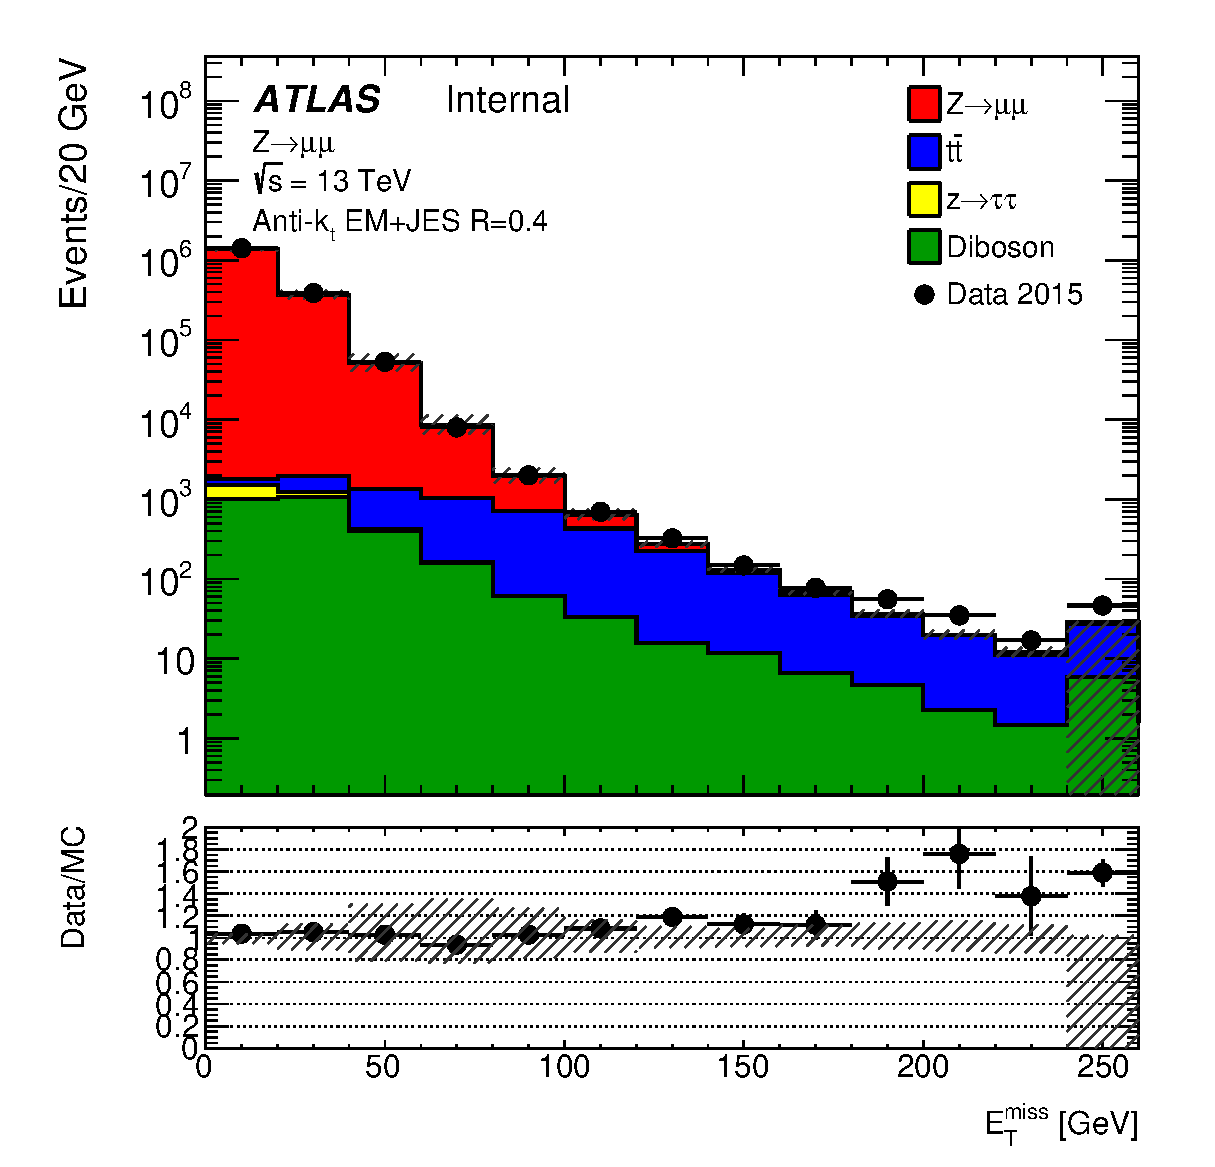
\includegraphics[width=\textwidth]{figures/zmumuStack_met.eps}
\caption{\met\ in a $Z\to ll$-rich region in data}
\label{fig:metPerfrunIIA}
\end{subfigure} % 
\begin{subfigure}{0.5\textwidth}
   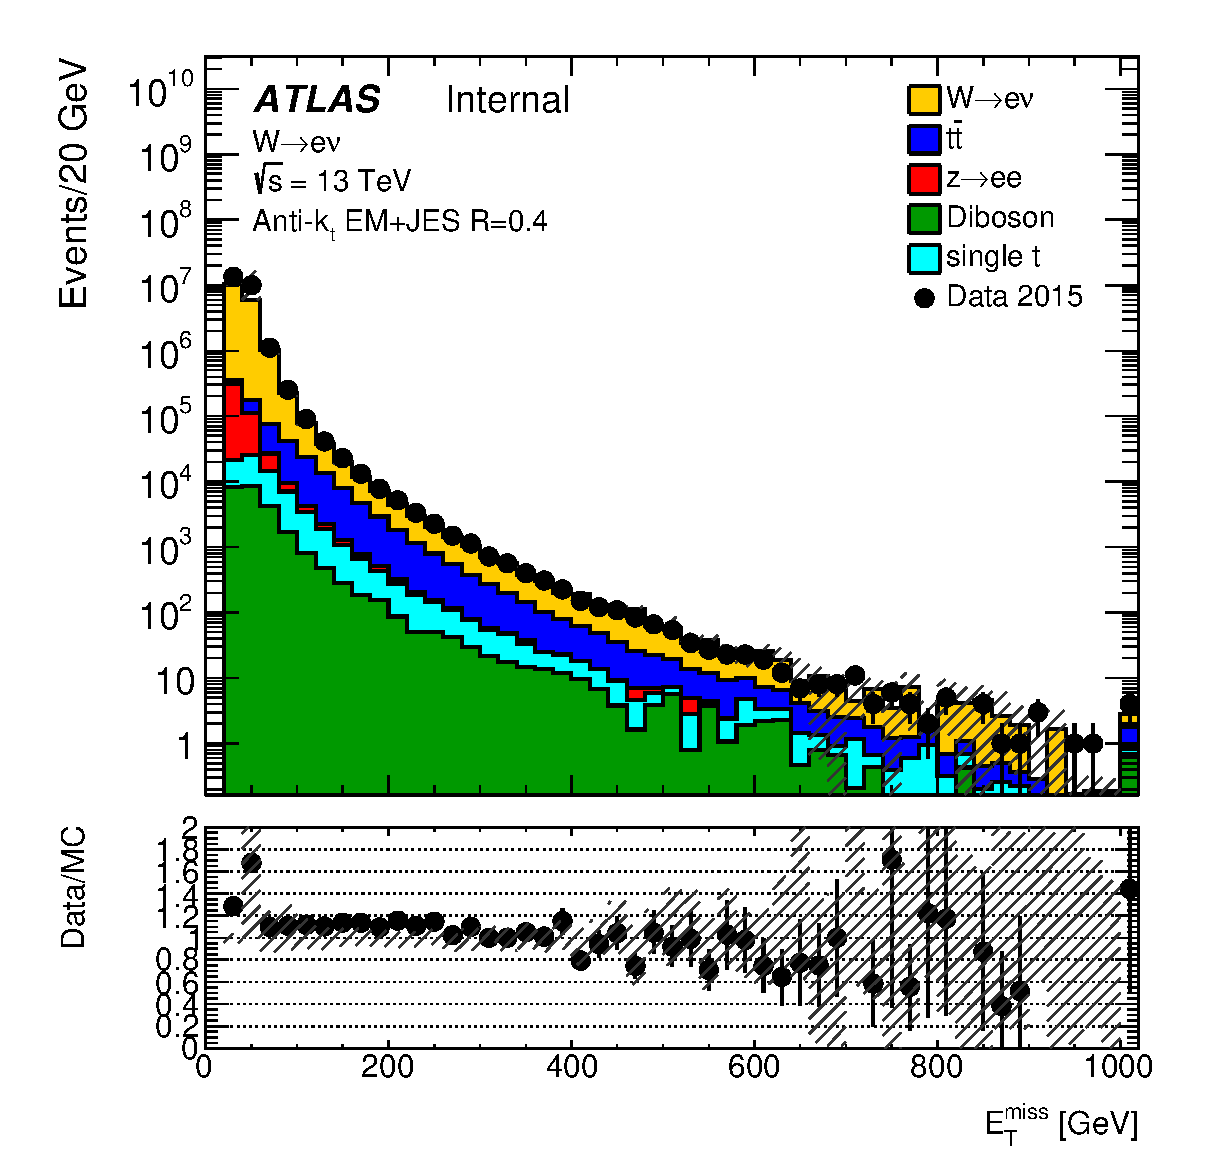
\includegraphics[width=\textwidth]{figures/wenuStack_met.eps}
\caption{\met\ in a $W\to l\nu$-rich region in data}
\label{fig:metPerfrunIIB}
\end{subfigure}
\caption{Plots showing distributions of \met\ in data, compared to predictions from Monte Carlo distributions, taken from 
Ref~\cite{Brunt:2149445}}
\end{figure}

\par Uncertainties on the \met\ scale were determined from comparisons between data and Monte Carlo
simulation. Alternative event generators were used. These were observed to be a few percent~\cite{Brunt:2149445}.


%\begin{chapsummary}
%Reconstruction of physics objects that are later used in Chapters~\ref{chargedH} and \ref{exclH} from the 
%ATLAS detector signals was discussed in this chapter. Photons were not discussed, but references were supplied. 
%Modelling of these reconstruction and identification schemes in Monte Carlo simulation was described, discussing any 
%necessary corrections that were applied. Evaluation of systematic uncertainties on each of these schemes was outlined, and 
%the sizes of the uncertainties were given.  
%\end{chapsummary}
